\documentclass[conference]{IEEEtran}
\IEEEoverridecommandlockouts
% The preceding line is only needed to identify funding in the first footnote. If that is unneeded, please comment it out.
\usepackage{cite, balance}
\usepackage{amsmath,amssymb,amsfonts}
\usepackage{algorithmic}
\usepackage[font=small,skip=0pt]{caption}
\DeclareMathOperator*{\argmax}{arg\,max}
\DeclareMathOperator*{\argmin}{arg\,min}
\newcommand{\bxi}{\boldsymbol{\xi}}
% for tikz
\usepackage[utf8]{inputenc}
\usepackage{pgfplots}
\DeclareUnicodeCharacter{2212}{−}
\usepgfplotslibrary{groupplots,dateplot}
\usetikzlibrary{patterns,shapes.arrows}
\pgfplotsset{compat=newest}
\pgfplotsset{every tick label/.append style={font=\tiny}}

% for algorithm
\usepackage[linesnumbered,ruled,vlined]{algorithm2e}
\usepackage{amssymb}
\usepackage{algorithmicx}
% \renewcommand{\algorithmicforall}{\textbf{for each}}

% for url
\usepackage{hyperref}
\hypersetup{
	colorlinks=true,
	linkcolor=blue,
	filecolor=magenta,      
	urlcolor=blue,
	pdftitle={Overleaf Example},
	pdfpagemode=FullScreen,
}
\urlstyle{same}

\usepackage{graphicx}
\usepackage{textcomp}
\usepackage{xcolor}
\def\BibTeX{{\rm B\kern-.05em{\sc i\kern-.025em b}\kern-.08em
		T\kern-.1667em\lower.7ex\hbox{E}\kern-.125emX}}
\begin{document}
	
	\title{Soft Fixtures: Practical Caging-Based Manipulation of Rigid and Deformable Objects
		\thanks{Funded by the European Commission under the Horizon Europe Framework Programme project SoftEnable, grant number 101070600, \url{http://softenable.eu/}.
			%Both authors are with the division of Robotics, Perception and Learning, 
			The authors are with the division of Robotics, Perception and Learning,
			KTH Royal Institute of Technology, Sweden, \{yifeid, fpokorny\}@kth.se.}
	}
	
	\author{
		\IEEEauthorblockN{Yifei Dong \and Florian T. Pokorny
		}
	}
	
	\maketitle
	
	\begin{abstract}
		We present a sampling-based approach and experiments to reasoning about the manipulation of both rigid and a simplified class of deformable objects, modeled as articulated rigid bodies with gravitational and elastic potential energy in 3D. We extend earlier work generalizing the notion of caging to include energy function constraints to allow for a quasi-static analysis and the inclusion of elastic potential energy of deformable objects. While past works on caging have predominantly focused on provably correct algorithms applicable to restricted simple classes of rigid objects such as polygons in 2D or simple meshes in 3D, our approach only provides upper bounds to escape energies, but in return allows for the analysis of such soft fixtures in much higher-dimensional configuration spaces. In this paper, we present demonstrations of simulation scenarios indicating that our approach can be applied to the analysis of escape energy for quasi-static manipulation scenarios involving rigid and articulated objects. Simulation results indicate that our proposed iterative or optimality-based search approaches provide a convincing and useful upper bound estimation of escape energy.
	\end{abstract}
	% The characteristics of caging grasps demonstrate advantages in handling delicate, irregular or deformable objects to assist human beings in industrial robot manipulation.
	%An object is caged by obstacles if it cannot escape arbitrarily far away.
	%Energy-bounded caging is a generalization of caging that considers the inclusion of energy constraints. 
	% allows for the tolerance of  escape paths with high energy costs.
	% It refers to trapping an object within a semi-closed free space partially bounded by obstacles in the presence of intrinsic or extrinsic forces. 
	%We propose a caging analysis approach that extends the state-of-the-art in several ways, including the analysis of 3D objects and obstacles, as well as different sources of bounding energy and various articulation of bodies.
	% 1. Caging analysis of 3D objects and obstacles of arbitrary shapes.
	% 2. Different sources of bounding energy - from external forces to internal elastic forces.
	% 3. Various types of bodies - from rigid to multi-joint articulated bodies.
	% We formulate the problem as randomly exploring the configuration space, building a potential energy map, and finding the optimal escape path.
	%To handle the high-dimensional configuration space of articulated objects in the presence of obstacles, a sampling-based approach and collision detection in a physics engine are used to implicitly approximate the free space.
	% almost-surely asymptotically optimal
	%To find an optimal escape path with minimum energy cost in the problem domain, an informed, anytime planner based on Batch Informed Trees (BIT*) with a configuration-cost function is presented. 
	%We implement the algorithm in Bullet and Open Motion Planning Library (OMPL) and empirically verify the BIT*-based approach with an iterative incremental search approach.
	%Initial experimented evaluation is presented in example scenarios, covering different body types, caging completeness, and complexity.
	%The results indicate the feasibility of applying our methods in high-dimensional articulated objects or approximated soft objects. 
	% The study provides complementary material, including videos with per-frame caging analysis and plots.
	
	
	\begin{IEEEkeywords}
		robotic manipulation, caging, sampling-based motion planning, potential energy
	\end{IEEEkeywords}
	
	
	\section{Introduction}
	The task of restraining an object, which is also referred to as fixturing, is one of the key
	functions of robotic grasping \cite{b18} and a key step towards robust dexterous manipulation.
	Enveloping grasps \cite{b19} effectively constrain objects by wrapping the fingers and palm around
	them, while fingertip grasps enable dexterous manipulation of objects with distal phalanges. While
	classical grasping approaches such as form and force closure \cite{b20} focus on the analysis of
	point-contacts with the goal of fully controlling the pose of a grasped object, these approaches,
	however, might suffer from grasp instability issues due to noise in perception and susceptibility to external disturbances. 
	
	Caging provides an alternative approach to fixturing, where the object is not necessarily fully immobilized. 
	% F. T. Pokorny, J. A. Stork, and D. Kragic, “Grasping objects with holes: A topological approach,” in ICRA, 2013, pp. 1100–1107.
	% ——, “A topology-based object representation for clasping, latching and hooking,” in HUMANOIDS, 2013.
	Caging by wrapping around objects and restricting their mobility provides a potential avenue to the fixture by taking advantage of the distal phalanges, the palm, or extrinsic dexterity \cite{b21} as additional constraints.
	Caging is a concept in which obstacles form a cage around an object, 
	% restricting its mobility without necessarily making contact with its surface. 
	and thus it requires the reasoning of objects' global attributes through configuration space, and the tolerance of bounded mobility makes it resistant to noise.
	%  unlike wrench space analysis which focuses on local contact characteristics.
	A potential advantage of caging we can envision is thus it allows a robot to fixture delicate or fragile objects without damaging them. 
	Caging could also be useful for grasping irregularly shaped objects that are difficult to grip using force closure grasps.
	% The advantages of caging grasps enable assistive robots to perform manipulation tasks in hazardous environments such as cold rooms, or in sanitization-demanding procedures. 
	% The tasks include handling delicate or soft items in the food industry such as meat and fish, as well as personal protective equipment in the medical industry such as masks, gowns, medical hats, etc.
	
	% \begin{figure}
		%     \centering
		%     \input{texs/hook-mosaic}
		%     % This file was created with tikzplotlib v0.10.1.
\begin{tikzpicture}

\definecolor{darkgray176}{RGB}{176,176,176}
\definecolor{lightgray204}{RGB}{204,204,204}
\definecolor{orangered2405932}{RGB}{240,59,32}
\definecolor{seagreen4916384}{RGB}{49,163,84}
\definecolor{slateblue117107177}{RGB}{117,107,177}
\definecolor{steelblue43140190}{RGB}{43,140,190}

\begin{groupplot}[group style={group size=3 by 2}]
\nextgroupplot[
tick pos=left,
title={B},
xmin=-0.5, xmax=1023.5,
y dir=reverse,
ymin=-0.5, ymax=1023.5
]
\addplot graphics [includegraphics cmd=\pgfimage,xmin=-0.5, xmax=1023.5, ymin=1023.5, ymax=-0.5] {ICRAfigure3-000.png};

\nextgroupplot[
tick pos=left,
title={A},
xmin=-0.5, xmax=1023.5,
y dir=reverse,
ymin=-0.5, ymax=1023.5
]
\addplot graphics [includegraphics cmd=\pgfimage,xmin=-0.5, xmax=1023.5, ymin=1023.5, ymax=-0.5] {ICRAfigure3-001.png};

\nextgroupplot[
tick pos=left,
title={D},
xmin=-0.5, xmax=1023.5,
y dir=reverse,
ymin=-0.5, ymax=1023.5
]
\addplot graphics [includegraphics cmd=\pgfimage,xmin=-0.5, xmax=1023.5, ymin=1023.5, ymax=-0.5] {ICRAfigure3-002.png};
\end{groupplot}

\begin{groupplot}[group style={group size=3 by 2}]
\nextgroupplot[
tick pos=left,
title={C},
xmin=-0.5, xmax=1023.5,
y dir=reverse,
ymin=-0.5, ymax=1023.5
]
\addplot graphics [includegraphics cmd=\pgfimage,xmin=-0.5, xmax=1023.5, ymin=1023.5, ymax=-0.5] {ICRAfigure3-003.png};

\nextgroupplot[
legend cell align={left},
legend style={fill opacity=0.8, draw opacity=1, text opacity=1, draw=lightgray204},
tick align=outside,
tick pos=left,
title={Escape energy plots},
x grid style={darkgray176},
xlabel={# iterations},
xmajorgrids,
xmin=-8.3, xmax=174.3,
xtick style={color=black},
y grid style={darkgray176},
ylabel={Potential energy},
ymajorgrids,
ymin=-1.57256743615714, ymax=29.673055592198,
ytick style={color=black}
]
\path [draw=orangered2405932, fill=orangered2405932, opacity=0.4]
(axis cs:0,0)
--(axis cs:0,0)
--(axis cs:1,0)
--(axis cs:2,0)
--(axis cs:3,0)
--(axis cs:4,0)
--(axis cs:5,0)
--(axis cs:6,0)
--(axis cs:7,-0.0647795153707492)
--(axis cs:8,-0.0158537986293012)
--(axis cs:9,-0.152311843959181)
--(axis cs:10,-0.0217982243533952)
--(axis cs:11,0.0263673753529359)
--(axis cs:12,0.262735278557434)
--(axis cs:13,0.195935264167078)
--(axis cs:14,1.00429079924269)
--(axis cs:15,1.21652942021891)
--(axis cs:16,0.227050384134112)
--(axis cs:17,1.40864334816279)
--(axis cs:18,1.35944038599191)
--(axis cs:19,2.50870484903156)
--(axis cs:20,2.72453973526567)
--(axis cs:21,2.96473018675072)
--(axis cs:22,2.92174736137564)
--(axis cs:23,3.19694285854262)
--(axis cs:24,3.465178536977)
--(axis cs:25,3.56191948371019)
--(axis cs:26,3.97441960049469)
--(axis cs:27,4.06895417489502)
--(axis cs:28,4.8306485240655)
--(axis cs:29,5.20724902652579)
--(axis cs:30,5.85085961488115)
--(axis cs:31,5.53499600535067)
--(axis cs:32,5.88717750230477)
--(axis cs:33,6.4267352988063)
--(axis cs:34,6.60931262266243)
--(axis cs:35,7.05469434101632)
--(axis cs:36,7.381013238661)
--(axis cs:37,7.7046138280853)
--(axis cs:38,8.16199719364059)
--(axis cs:39,8.43394342712708)
--(axis cs:40,8.69389935083448)
--(axis cs:41,8.5149198848057)
--(axis cs:42,8.64793476926026)
--(axis cs:43,8.89959907816296)
--(axis cs:44,8.83907425083114)
--(axis cs:45,8.3001576602444)
--(axis cs:46,8.70537058858776)
--(axis cs:47,8.8464393192841)
--(axis cs:48,8.2470678337009)
--(axis cs:49,8.80906582996363)
--(axis cs:50,8.54741458784685)
--(axis cs:51,9.1463898267305)
--(axis cs:52,8.75710656331347)
--(axis cs:53,9.44557747258025)
--(axis cs:54,9.43791384173197)
--(axis cs:55,8.96258443904128)
--(axis cs:56,9.19591923356461)
--(axis cs:57,9.02470630514324)
--(axis cs:58,8.85658182643551)
--(axis cs:59,8.9212952716248)
--(axis cs:60,9.5896598884376)
--(axis cs:61,9.40583871770402)
--(axis cs:62,9.85224861632557)
--(axis cs:63,9.56465178792056)
--(axis cs:64,9.4134206181347)
--(axis cs:65,9.69618819308817)
--(axis cs:66,9.27151906329271)
--(axis cs:67,9.48855848293231)
--(axis cs:68,9.77232053049905)
--(axis cs:69,9.26428137541625)
--(axis cs:70,9.35618854581132)
--(axis cs:71,9.42804542659066)
--(axis cs:72,10.0209079112007)
--(axis cs:73,10.0216934066963)
--(axis cs:74,10.0971033654415)
--(axis cs:75,10.056446938598)
--(axis cs:76,9.93852471430816)
--(axis cs:77,10.2336460267426)
--(axis cs:78,10.3409365806773)
--(axis cs:79,10.4624632084561)
--(axis cs:80,10.3709731178522)
--(axis cs:81,10.5972577660694)
--(axis cs:82,10.4889723896803)
--(axis cs:83,10.4555976257636)
--(axis cs:84,10.4119974839198)
--(axis cs:85,10.7027642782004)
--(axis cs:86,10.8648129477242)
--(axis cs:87,10.6128444363664)
--(axis cs:88,10.189013602568)
--(axis cs:89,11.1161994086985)
--(axis cs:90,10.8175708742596)
--(axis cs:91,11.1564722705895)
--(axis cs:92,11.3023712542417)
--(axis cs:93,10.8409924203978)
--(axis cs:94,11.0628565949691)
--(axis cs:95,11.0103350385368)
--(axis cs:96,11.4529732254085)
--(axis cs:97,11.1105961015774)
--(axis cs:98,10.9946741645954)
--(axis cs:99,11.0845571296184)
--(axis cs:100,11.1294948693354)
--(axis cs:101,11.196655236346)
--(axis cs:102,11.0354870758315)
--(axis cs:103,11.3906313924325)
--(axis cs:104,10.8941212449424)
--(axis cs:105,11.1648505374371)
--(axis cs:106,10.6725299497703)
--(axis cs:107,11.1462058865047)
--(axis cs:108,11.3530912855322)
--(axis cs:109,10.6639112332071)
--(axis cs:110,10.7773227447953)
--(axis cs:111,11.4107408659931)
--(axis cs:112,11.4237508020925)
--(axis cs:113,11.1382242102848)
--(axis cs:114,10.6921256402185)
--(axis cs:115,11.0916068898524)
--(axis cs:116,10.9231260545476)
--(axis cs:117,11.4913419618229)
--(axis cs:118,11.0541231486434)
--(axis cs:119,11.2348668593489)
--(axis cs:120,11.4020737447213)
--(axis cs:121,10.9958469896178)
--(axis cs:122,11.4215437708682)
--(axis cs:123,11.1070165041418)
--(axis cs:124,11.6578901804967)
--(axis cs:125,11.1377018187012)
--(axis cs:126,11.9235251529536)
--(axis cs:127,11.6960197358746)
--(axis cs:128,11.4042217321005)
--(axis cs:129,11.2797979667541)
--(axis cs:130,11.3991030796662)
--(axis cs:131,11.1296240049966)
--(axis cs:132,12.163341958577)
--(axis cs:133,11.865903295924)
--(axis cs:134,11.5311350014202)
--(axis cs:135,12.0381455025606)
--(axis cs:136,12.0327328994821)
--(axis cs:137,12.5489258447257)
--(axis cs:138,11.9577099805342)
--(axis cs:139,11.9748120203984)
--(axis cs:140,11.7906137081884)
--(axis cs:141,12.0208742089521)
--(axis cs:142,12.4104420833029)
--(axis cs:143,11.8526631790756)
--(axis cs:144,11.8688508226856)
--(axis cs:145,11.8075612181612)
--(axis cs:146,11.7200630963902)
--(axis cs:147,11.2864130028464)
--(axis cs:148,11.9504587365586)
--(axis cs:149,12.1339761891776)
--(axis cs:150,11.5679429040657)
--(axis cs:151,11.471055359893)
--(axis cs:152,11.8519138597865)
--(axis cs:153,11.9068318347074)
--(axis cs:154,11.7481177884074)
--(axis cs:155,11.8644169699635)
--(axis cs:156,11.4600399741989)
--(axis cs:157,11.8425138892686)
--(axis cs:158,12.2107167800222)
--(axis cs:159,11.8275669689193)
--(axis cs:160,12.020375887091)
--(axis cs:161,12.1656713093505)
--(axis cs:162,11.9728096502625)
--(axis cs:163,11.8189354775159)
--(axis cs:164,11.8341371213149)
--(axis cs:165,11.4385436532553)
--(axis cs:166,11.6408868919448)
--(axis cs:166,12.6659206669685)
--(axis cs:166,12.6659206669685)
--(axis cs:165,12.2867720733433)
--(axis cs:164,12.4782057991057)
--(axis cs:163,12.4217842249858)
--(axis cs:162,12.5198707138338)
--(axis cs:161,12.7671429816962)
--(axis cs:160,12.5661657419536)
--(axis cs:159,12.6118947918428)
--(axis cs:158,12.3259004323217)
--(axis cs:157,12.6523834030274)
--(axis cs:156,11.9946271989283)
--(axis cs:155,12.3784692574984)
--(axis cs:154,12.4422412846541)
--(axis cs:153,12.7664440766808)
--(axis cs:152,12.4391474053753)
--(axis cs:151,12.4976099640337)
--(axis cs:150,12.6779117033365)
--(axis cs:149,12.5378125031068)
--(axis cs:148,12.840980127242)
--(axis cs:147,12.3964279132227)
--(axis cs:146,12.3248104066561)
--(axis cs:145,12.909245001997)
--(axis cs:144,12.8804744840638)
--(axis cs:143,12.4766970626908)
--(axis cs:142,12.6575586422085)
--(axis cs:141,12.4365451743891)
--(axis cs:140,12.5182726869471)
--(axis cs:139,13.0388155854813)
--(axis cs:138,12.5679719949073)
--(axis cs:137,13.0266619286417)
--(axis cs:136,12.4360622802556)
--(axis cs:135,12.4613346363975)
--(axis cs:134,12.4803146234102)
--(axis cs:133,12.6692986769494)
--(axis cs:132,12.6148578657367)
--(axis cs:131,12.5392765633907)
--(axis cs:130,12.3237922450841)
--(axis cs:129,12.7313521719599)
--(axis cs:128,12.3729700045202)
--(axis cs:127,12.2801464459229)
--(axis cs:126,12.3857512093994)
--(axis cs:125,12.260034123225)
--(axis cs:124,12.243902713455)
--(axis cs:123,11.7306225228046)
--(axis cs:122,12.1096162647251)
--(axis cs:121,11.9153640947748)
--(axis cs:120,11.9608871996942)
--(axis cs:119,11.8892750309545)
--(axis cs:118,11.9345658564046)
--(axis cs:117,12.0740182967845)
--(axis cs:116,11.5980350825257)
--(axis cs:115,12.0383511835627)
--(axis cs:114,11.9491240308573)
--(axis cs:113,11.8416256253005)
--(axis cs:112,11.7257662548838)
--(axis cs:111,12.1354894989017)
--(axis cs:110,11.5027158704497)
--(axis cs:109,11.4668038549421)
--(axis cs:108,11.919779884863)
--(axis cs:107,11.7329649644848)
--(axis cs:106,12.1700728200521)
--(axis cs:105,11.672887194767)
--(axis cs:104,11.9183152271051)
--(axis cs:103,11.9698598835237)
--(axis cs:102,11.9177030505822)
--(axis cs:101,11.5961395101561)
--(axis cs:100,11.6122332275858)
--(axis cs:99,12.0180944197035)
--(axis cs:98,11.8158407346749)
--(axis cs:97,11.6473397276936)
--(axis cs:96,11.9666700404463)
--(axis cs:95,11.3678924180867)
--(axis cs:94,11.5326175798775)
--(axis cs:93,11.734098391761)
--(axis cs:92,11.5575591927674)
--(axis cs:91,11.6799729100391)
--(axis cs:90,11.5511342120712)
--(axis cs:89,11.6208543521704)
--(axis cs:88,11.5548444208349)
--(axis cs:87,11.1894178426987)
--(axis cs:86,11.7659439237223)
--(axis cs:85,11.3192868716113)
--(axis cs:84,11.5514115508407)
--(axis cs:83,11.6205786022468)
--(axis cs:82,10.9426246895168)
--(axis cs:81,11.1458356078924)
--(axis cs:80,11.0824658356166)
--(axis cs:79,11.0100113022293)
--(axis cs:78,10.8924373585598)
--(axis cs:77,11.1985062669906)
--(axis cs:76,10.9316103593625)
--(axis cs:75,10.4956697230909)
--(axis cs:74,10.7957150595133)
--(axis cs:73,10.5577346016138)
--(axis cs:72,10.5101499379871)
--(axis cs:71,10.5539788199116)
--(axis cs:70,10.5885598583879)
--(axis cs:69,10.227162125045)
--(axis cs:68,10.5761012524675)
--(axis cs:67,10.0414034207366)
--(axis cs:66,10.2663223779576)
--(axis cs:65,10.5559124665187)
--(axis cs:64,10.3350893223153)
--(axis cs:63,10.4571669243025)
--(axis cs:62,10.3515206191248)
--(axis cs:61,10.0490534762548)
--(axis cs:60,10.1093649972765)
--(axis cs:59,9.68714109469701)
--(axis cs:58,9.87371031126691)
--(axis cs:57,9.75711449050184)
--(axis cs:56,9.7108505897837)
--(axis cs:55,9.87932669183459)
--(axis cs:54,10.2216026574794)
--(axis cs:53,9.86501880138657)
--(axis cs:52,9.41739999708111)
--(axis cs:51,9.70314635950491)
--(axis cs:50,9.97928030631053)
--(axis cs:49,9.89542795176421)
--(axis cs:48,8.79461969820438)
--(axis cs:47,9.40019326959885)
--(axis cs:46,9.57203061999093)
--(axis cs:45,8.96817752552063)
--(axis cs:44,9.38498625620264)
--(axis cs:43,9.54426090909922)
--(axis cs:42,9.79211745694365)
--(axis cs:41,9.66751104443427)
--(axis cs:40,9.45421883248397)
--(axis cs:39,9.10945027156758)
--(axis cs:38,8.44240574600929)
--(axis cs:37,8.66677642592168)
--(axis cs:36,8.05566053341573)
--(axis cs:35,7.54091164519573)
--(axis cs:34,7.24423994876992)
--(axis cs:33,6.963564594862)
--(axis cs:32,6.69718941027319)
--(axis cs:31,6.2926475922601)
--(axis cs:30,5.95685757167174)
--(axis cs:29,5.65840500954406)
--(axis cs:28,5.3287687225649)
--(axis cs:27,5.11945373503714)
--(axis cs:26,4.68013215046011)
--(axis cs:25,4.68158003435945)
--(axis cs:24,3.95931779585954)
--(axis cs:23,3.60476362903545)
--(axis cs:22,3.79637700155408)
--(axis cs:21,3.56279271172453)
--(axis cs:20,3.03212368680035)
--(axis cs:19,3.0366984710051)
--(axis cs:18,2.44743274630549)
--(axis cs:17,1.90465923111513)
--(axis cs:16,2.03280249179549)
--(axis cs:15,1.88022246589462)
--(axis cs:14,1.63805633437751)
--(axis cs:13,0.928227198640385)
--(axis cs:12,0.610882074542631)
--(axis cs:11,0.418534054625991)
--(axis cs:10,0.301492921295694)
--(axis cs:9,0.510504095797925)
--(axis cs:8,0.0475613958879037)
--(axis cs:7,0.194338546112247)
--(axis cs:6,0)
--(axis cs:5,0)
--(axis cs:4,0)
--(axis cs:3,0)
--(axis cs:2,0)
--(axis cs:1,0)
--(axis cs:0,0)
--cycle;

\addplot [thick, seagreen4916384]
table {%
0 28.2528
1 28.2407719059961
2 28.2107098329643
3 28.162626110738
4 28.0965352669655
5 28.0124540201387
6 27.9104012715597
7 27.7903980962539
8 27.6524677328385
9 27.4966355723572
10 27.3229291460923
11 27.1313781123663
12 26.922014242347
13 26.69487140487
14 26.4499855502943
15 26.1873946934066
16 25.9071388953931
17 25.6092602448937
18 25.2938028381619
19 24.9608127583451
20 24.6523211434394
21 24.4166500808067
22 24.1739782398404
23 23.9281155249988
24 23.6749233487674
25 23.4138377667473
26 23.1436671659668
27 22.8644790486277
28 22.574006194248
29 22.2696498318469
30 21.954258770756
31 21.6375298060636
32 21.3112099868662
33 20.975949672904
34 20.6316503174314
35 20.2781797568087
36 19.915371595589
37 19.5430296198652
38 19.1605791740546
39 18.7686847297257
40 18.5048507730097
41 18.4076499791101
42 18.3714455451852
43 18.3723682150292
44 18.3765027516668
45 18.3770256589323
46 18.398027176176
47 18.3561882637977
48 18.2781283265859
49 18.2092656828487
50 18.145981888197
51 18.0858792524718
52 18.027411509755
53 17.9695749787236
54 17.9117030748669
55 17.8532776804778
56 17.8290121445491
57 17.8172596927886
58 17.8007855646607
59 17.7704283238606
60 17.7290459194855
61 17.6886416766615
62 17.6437885692207
63 17.6054332303512
64 17.5807734329771
65 17.579444327086
66 17.5442676808494
67 17.4820606329714
68 17.4390210998405
69 17.3985120512728
70 17.3552843112667
71 17.3081388976145
72 17.2502084591251
73 17.1810136880288
74 17.1012489043628
75 17.0117116201043
76 16.9726840253839
77 16.9422242946731
78 16.8966531843007
79 16.8384069593434
80 16.7689976027953
81 16.7022096813145
82 16.6320374585856
83 16.5488809802064
84 16.4540070995884
85 16.3686578344835
86 16.3427350700154
87 16.3481511834166
88 16.3305219783172
89 16.290852323229
90 16.2452967594126
91 16.2243348293519
92 16.2188132434189
93 16.2304277903298
94 16.2214674269417
95 16.185912151059
96 16.1329656433229
97 16.0969469116183
98 16.0742907514501
99 16.0782003422049
100 16.0827988620908
101 16.0737632019432
102 16.0534115017766
103 16.0311945050392
104 16.011352046116
105 15.9934018351407
106 15.9996779943348
107 16.001532102273
108 15.9962430245432
109 15.989335037805
110 15.9996311237186
111 16.0006517890161
112 15.9920703696771
113 15.9787529247034
114 15.9679707239816
115 15.9654701878795
116 15.9544720609103
117 15.9383383034323
118 15.9207394058294
119 15.9057658450369
120 15.8884123150917
121 15.8678342283046
122 15.8383383753631
123 15.8072198282125
124 15.7739706863686
125 15.7408787324768
126 15.7045420933851
127 15.6683829316288
128 15.6314418806651
129 15.5930170274546
130 15.5530981720251
131 15.5115555164485
132 15.4686163998126
133 15.4243095239922
134 15.3787796583265
135 15.3323586230065
136 15.284920934225
137 15.2365548903079
138 15.1876116053946
139 15.1382274223986
140 15.1415985370732
141 15.1723273844127
142 15.1962637749664
143 15.2170664642479
144 15.2365086657724
145 15.2554752759206
146 15.2743931867324
147 15.2934664783478
148 15.3127886722109
149 15.3244687176829
150 15.3232181944705
151 15.3221300458703
152 15.3211242073363
153 15.320207558046
154 15.3193475855486
155 15.3185144833647
156 15.3177087535494
157 15.3169397158531
158 15.316213007676
159 15.3155305769447
160 15.3148937551837
161 15.314303834245
162 15.3137613750228
163 15.3132647350068
164 15.3127802271503
165 15.3122858488427
166 15.311848450884
};
\addlegendentry{Total energy}
\addplot [semithick, slateblue117107177, dashed]
table {%
0 28.2528
1 28.2407719059961
2 28.2107098329643
3 28.162626110738
4 28.0965352669655
5 28.0124540201387
6 27.9104012715597
7 27.7903980962539
8 27.6524677328385
9 27.4966355723572
10 27.3229291460923
11 27.1313781123663
12 26.922014242347
13 26.69487140487
14 26.4499855502943
15 26.1873946934066
16 25.9071388953931
17 25.6092602448937
18 25.2938028381619
19 24.9608127583451
20 24.6482584727062
21 24.4082013532825
22 24.1617188465115
23 23.9120310332695
24 23.6554801733771
25 23.3912395123192
26 23.1182085606524
27 22.8360866390482
28 22.5434845260135
29 22.2380756789324
30 21.9213243409399
31 21.6010243217883
32 21.2720909373463
33 20.9346169263338
34 20.5884149289865
35 20.233328973151
36 19.8691897674121
37 19.4958039577817
38 19.1127014395691
39 18.7202251466854
40 18.4029463608915
41 18.1664807537624
42 17.9584226895637
43 17.7689034175464
44 17.5875713921058
45 17.4084021278994
46 17.2364442075538
47 17.1042727251597
48 16.999673070592
49 16.9046725914481
50 16.8154402922086
51 16.7295812198101
52 16.6454241035619
53 16.5617582179972
54 16.4776888171104
55 16.3925174525621
56 16.316584207227
57 16.2496177137777
58 16.1839288850563
59 16.1137624682459
60 16.0389518053697
61 15.9776883334788
62 15.9152289386265
63 15.8578074360093
64 15.8144566685222
65 15.7823468316359
66 15.7278949039877
67 15.653062724292
68 15.5962846674812
69 15.5375317207012
70 15.475865116989
71 15.4101663021687
72 15.3371730757895
73 15.2560033668501
74 15.1660556087384
75 15.0672862508584
76 15.0085456752212
77 14.9536698901314
78 14.890929136285
79 14.8199882666485
80 14.740620773629
81 14.6753396956038
82 14.6021276781234
83 14.5186256003921
84 14.4248661946526
85 14.3310708213714
86 14.2729869405926
87 14.2275691157652
88 14.1737943212306
89 14.1187386273456
90 14.0781585473486
91 14.0618825917664
92 14.0519085753968
93 14.0480616626819
94 14.0262289745512
95 13.9851185690902
96 13.9380879496471
97 13.9137966311753
98 13.9114295021967
99 13.9160710764582
100 13.9209096806241
101 13.9227548706632
102 13.9379671605673
103 13.9544689145716
104 13.9720737948367
105 13.990546728593
106 14.016618048278
107 14.0390615841313
108 14.05807528032
109 14.0759734663327
110 14.0985012473413
111 14.1155433523477
112 14.1272345967546
113 14.1363816256813
114 14.1464899755001
115 14.1576631517312
116 14.16500526396
117 14.1695569051556
118 14.1733529403843
119 14.1688656823952
120 14.1477730752009
121 14.1334302164847
122 14.1071714271844
123 14.0927812789043
124 14.0776101491069
125 14.0607820309293
126 14.0410302789487
127 14.0203601243407
128 13.9980587270964
129 13.9739995487622
130 13.9482813238208
131 13.9210606078448
132 13.8924624024673
133 13.8626928277067
134 13.8318765436407
135 13.8000988634604
136 13.7674838869829
137 13.7341216769957
138 13.7000965126793
139 13.6654850497495
140 13.6381830901665
141 13.6218814040109
142 13.6094034820633
143 13.5987345138225
144 13.5888888319313
145 13.5793959323764
146 13.5700425775191
147 13.5607332112355
148 13.5514266825214
149 13.543033015261
150 13.5389874491138
151 13.5356815937989
152 13.5325397001798
153 13.5294434658649
154 13.5263453837569
155 13.5232267249356
156 13.5200875476797
157 13.5169331932419
158 13.5137666499925
159 13.510589251226
160 13.5074019130498
161 13.5042057346807
162 13.5010017217911
163 13.4977920256187
164 13.4945819408599
165 13.491371119493
166 13.4881640784413
};
\addlegendentry{Gravity potential energy}
\addplot [semithick, steelblue43140190, dashed]
table {%
0 0
1 2.88069519478737e-35
2 4.58895608396853e-35
3 1.60138969722821e-34
4 1.83651701990349e-34
5 3.59179295944918e-34
6 4.40739392523361e-34
7 7.3537892829087e-34
8 1.0557667626888e-33
9 1.33085357431898e-33
10 2.12795226767818e-33
11 3.36522907613033e-33
12 4.58496143195924e-33
13 5.72648313631534e-33
14 6.8445128089861e-33
15 7.85072106067208e-33
16 9.2908486341233e-33
17 1.13369270357809e-32
18 1.34458836858991e-32
19 1.65606350599171e-32
20 0.00406267073316435
21 0.00844872752426503
22 0.0122593933289266
23 0.0160844917292727
24 0.0194431753903181
25 0.0225982544281086
26 0.0254586053144535
27 0.0283924095794657
28 0.0305216682344901
29 0.0315741529145665
30 0.0329344298161645
31 0.0365054842752388
32 0.0391190495199076
33 0.0413327465701905
34 0.0432353884449315
35 0.0448507836577296
36 0.0461818281769109
37 0.0472256620834533
38 0.0478777344855136
39 0.0484595830403349
40 0.101904412118153
41 0.241169225347697
42 0.413022855621543
43 0.603464797482848
44 0.788931359560986
45 0.968623531032913
46 1.16158296862221
47 1.25191553863798
48 1.27845525599395
49 1.30459309140062
50 1.33054159598835
51 1.35629803266172
52 1.38198740619314
53 1.40781676072643
54 1.43401425775652
55 1.46076022791564
56 1.51242793732201
57 1.56764197901099
58 1.61685667960435
59 1.65666585561465
60 1.69009411411581
61 1.71095334318275
62 1.7285596305942
63 1.74762579434194
64 1.76631676445489
65 1.79709749545007
66 1.81637277686172
67 1.82899790867939
68 1.84273643235925
69 1.86098033057159
70 1.87941919427771
71 1.89797259544582
72 1.91303538333558
73 1.92501032117872
74 1.9351932956244
75 1.94442536924587
76 1.9641383501627
77 1.98855440454171
78 2.00572404801575
79 2.0184186926949
80 2.02837682916626
81 2.02686998571066
82 2.02990978046223
83 2.03025537981433
84 2.02914090493576
85 2.03758701311214
86 2.06974812942274
87 2.12058206765137
88 2.15672765708662
89 2.17211369588337
90 2.16713821206393
91 2.16245223758541
92 2.16690466802203
93 2.1823661276479
94 2.19523845239052
95 2.20079358196886
96 2.19487769367578
97 2.18315028044298
98 2.1628612492534
99 2.16212926574668
100 2.16188918146668
101 2.15100833127998
102 2.11544434120929
103 2.07672559046762
104 2.03927825127927
105 2.00285510654778
106 1.98305994605681
107 1.96247051814172
108 1.93816774422316
109 1.91336157147231
110 1.90112987637736
111 1.88510843666842
112 1.8648357729225
113 1.84237129902212
114 1.82148074848155
115 1.80780703614821
116 1.78946679695028
117 1.76878139827669
118 1.74738646544506
119 1.73690016264166
120 1.74063923989087
121 1.73440401181983
122 1.73116694817873
123 1.71443854930815
124 1.69636053726173
125 1.68009670154759
126 1.66351181443641
127 1.64802280728808
128 1.63338315356867
129 1.61901747869234
130 1.60481684820429
131 1.59049490860365
132 1.57615399734538
133 1.56161669628554
134 1.54690311468582
135 1.53225975954615
136 1.51743704724212
137 1.50243321331219
138 1.48751509271534
139 1.47274237264909
140 1.50341544690675
141 1.55044598040187
142 1.58686029290307
143 1.61833195042541
144 1.64761983384109
145 1.67607934354415
146 1.70435060921333
147 1.73273326711233
148 1.76136198968948
149 1.78143570242191
150 1.78423074535663
151 1.78644845207136
152 1.78858450715649
153 1.79076409218101
154 1.79300220179167
155 1.79528775842906
156 1.7976212058697
157 1.80000652261127
158 1.80244635768343
159 1.80494132571871
160 1.80749184213385
161 1.81009809956432
162 1.81275965323173
163 1.81547270938805
164 1.81819828629034
165 1.82091472934973
166 1.82368437244271
};
\addlegendentry{Elastic potential energy}
\addplot [thick, orangered2405932]
table {%
0 0
1 0
2 0
3 0
4 0
5 0
6 0
7 0
8 0
9 0
10 0
11 0
12 0.289915982756376
13 0
14 0.705379585399566
15 1.11704575966591
16 0
17 1.33370285806742
18 1.27854285869392
19 2.51604679060868
20 2.69625320471152
21 2.91928641508458
22 2.56979202029162
23 3.08624422409042
24 3.3564899071007
25 3.11746288658712
26 3.86269635604603
27 3.58713817165762
28 4.73438326913897
29 5.2703939688831
30 5.8170871857067
31 5.34539648095371
32 5.92607980561977
33 6.20707934309173
34 6.34870750143081
35 6.9407694322126
36 7.24999286493149
37 7.29771792202497
38 8.16184702441174
39 8.36486690357135
40 8.55319314367457
41 8.43588416706651
42 8.44067684108647
43 8.70224422720246
44 8.7349187077487
45 8.11002993703919
46 8.4660014835943
47 8.67270267256697
48 8.1242301447341
49 8.34562621936681
50 7.94361045151399
51 9.05756700480457
52 8.50134818318688
53 9.316076258642
54 9.34921241908487
55 8.74891912769143
56 9.11654799232151
57 8.83237284068518
58 8.7544900965185
59 8.81671469951726
60 9.45144199313667
61 9.19497479629794
62 9.86084391352914
63 9.14511602509018
64 9.3758858432203
65 9.64776408194062
66 9.05495813607437
67 9.40674854952413
68 9.51583149289159
69 9.17256208954447
70 9.05771443400835
71 9.27873998624973
72 10.0442386243203
73 10.014152155448
74 10.041409427033
75 9.88732018524363
76 9.96423002957059
77 10.1149120790407
78 10.3339687825584
79 10.2064679987049
80 10.1329252307426
81 10.6129146643152
82 10.2773904968339
83 10.2597469791325
84 10.0455182204462
85 10.5333946516088
86 10.600028414583
87 10.5822637732587
88 9.54607959806596
89 10.8985360510567
90 10.500155819693
91 10.9728208611761
92 11.2773188288583
93 10.7316864525358
94 11.0048011390651
95 10.9991781611188
96 11.3306673292893
97 11.1269767465272
98 10.7596648362878
99 11.0116021789509
100 11.0407555867267
101 11.1399409641328
102 10.6187074250243
103 11.2111693165722
104 10.6897465152634
105 11.1639143818029
106 10.3544786143411
107 11.0105113968476
108 11.2777079068694
109 10.5250104972107
110 10.6286811587599
111 11.0783514504679
112 11.3687737668123
113 11.0900748131917
114 10.2540162089559
115 10.7798738043565
116 10.8048937149378
117 11.3563986456779
118 10.7475371715445
119 11.2231128555562
120 11.2177401183995
121 10.5566443019257
122 11.1977681983913
123 11.0031908233459
124 11.473521918174
125 10.9210390843029
126 11.7161073799799
127 11.4291975591638
128 11.1705045496394
129 10.6356650358036
130 11.2807822771272
131 10.481182534558
132 12.1054075051384
133 11.826590455451
134 11.2389852751152
135 12.0455703116931
136 11.8661228345697
137 12.5627027038129
138 11.7108076005479
139 11.5798798930546
140 11.7156282774971
141 11.908156336087
142 12.4120872104145
143 11.7377893949109
144 11.7442209627133
145 11.6887301359445
146 11.5373332308414
147 11.4002835354476
148 11.5745638972535
149 12.1362786969118
150 11.5551079342833
151 11.0565695867608
152 11.8678430866064
153 11.5484390376135
154 11.7734475598287
155 11.8777842604881
156 11.3426291244439
157 11.6720593899184
158 12.1895410325048
159 11.6623343801271
160 11.8555731047324
161 12.0331633759633
162 11.7388329107932
163 11.5671184098723
164 11.7932082887104
165 11.2820217244824
166 11.5823230298255
};
\addlegendentry{Escape energy cost}
\addplot [black, dashed, forget plot]
table {%
2.00000000000001 -1.57256743615714
2.00000000000001 29.673055592198
};
\addplot [black, dashed, forget plot]
table {%
28 -1.57256743615714
28 29.673055592198
};
\addplot [black, dashed, forget plot]
table {%
88 -1.57256743615714
88 29.673055592198
};
\addplot [black, dashed, forget plot]
table {%
155 -1.57256743615714
155 29.673055592198
};
\draw (axis cs:2.5,-0.1) node[
  scale=0.9,
  anchor=base west,
  text=black,
  rotate=0.0
]{A};
\draw (axis cs:28.5,-0.1) node[
  scale=0.9,
  anchor=base west,
  text=black,
  rotate=0.0
]{B};
\draw (axis cs:88.5,-0.1) node[
  scale=0.9,
  anchor=base west,
  text=black,
  rotate=0.0
]{C};
\draw (axis cs:155.5,-0.1) node[
  scale=0.9,
  anchor=base west,
  text=black,
  rotate=0.0
]{D};
\end{groupplot}

\end{tikzpicture}

		%     % \vspace{-10pt}
		%     \caption{
			%     Quasi-static soft fixture analysis of two simulated dynamic scenes of a rigid ring under gravity (top) and a deformable fish model falling into a bowl (bottom). We display total potential energy (green), gravitational potential energy (purple), elastic potential energy (blue), and estimated required soft fixture escape energy (red) for each frame. Escape energy is estimated using 5 independent runs of a 2-min execution of the BIT*-based escape energy approximation.}
		%     % Each iteration is repeated 5 times independently.
		%     % the green curves denote the total potential energy of the caged objects, the red curves the minimum of escape energy costs over $6$ runs, with
		%     %The plus/minus one standard deviation of the escape energy costs extends from its mean (not plotted since we care about the minimum only, which is closest to and upper-bounds the optimal escape energy costs $u^* = V(\sigma^*) $) in red shadings. }
	%     \label{fig1}
	%     % \vspace{-19pt}
	% \end{figure}

In this work, we present progress on further extending the notion of caging to what we refer to as a \textbf{soft fixture}, where an object is constrained to a bounded path-component within a sublevel set of a suitable constraint function.
We in particular explore constraints imposed by the sublevel set of a function defined in terms of potential energy for this purpose. 
Unlike computationally expensive volumetric approximations of configuration space such as 3D rigid body caging using the methods of \cite{x1}, which currently cannot be applied in higher-dimensional configuration spaces or dynamic scenarios, we utilize a sampling-based approach that we show is applicable even to deformable objects approximately modeled as articulated objects.

Our primary contributions include 1) A generalization of 2D energy-bounded caging of rigid objects towards high-dimensional 3D rigid or deformable objects soft fixture in terms of a potential energy-based constraint function; 
2) Sampling-based algorithms that give an estimated upper bound of escape energy; 
3) Analysis of escape energy in manipulation primitives of practical scenarios ranging from fields of food processing and health care that cover various rigid or deformable objects, as well as simple evaluation in a physical experiment.
Demonstrations of such soft fixtures and their quasi-static analysis are implemented in the experiment\footnote{A video is available here: \url{https://youtu.be/tnYr7MSPMTw}}.
% J. Mahler, F. T. Pokorny, Z. McCarthy, A. F. van der Stappen, and K. Goldberg, “Energy-bounded caging: Formal definition and 2-d energy lower bound algorithm based on weighted alpha shapes,” IEEE Robotics and Automation Letters, vol. 1, no. 1, pp. 508–515, 2016.
% J. Mahler, F. T. Pokorny, S. Niyaz, and K. Goldberg, “Synthesis of energy-bounded planar caging grasps using persistent homology,” IEEE Transactions on Automation Science and Engineering, 2018.
%Our approach in particular builds on the concept of energy-bounded caging is an inter-body behavior that we frequently see in daily life such as a smartphone held in hand or keys in the pocket.

%In these scenarios, a target object is partially surrounded by obstacles and securely stays within the neighborhood of a local minimum of an energy function.
%The partial caging is assumed unbreakable unless external energy above a threshold is provided.
% The escape path that leads the caged object out of the trap usually passes through a saddle point in the configuration space.
%The energy bound plays an important role and we usually want to maximize it in order to form a robust cage against disturbances.
% transport a glass of water from point A to B

% \vspace{-2pt}
\section{Related Work}

\subsection{Caging Grasps}
The notion of caging was introduced by Kuperberg\cite{b1} as the problem of preventing a polygon from escaping arbitrarily far away using a set of fixed point-obstacles. More precisely, an object configuration is caged if its path-component in collision-free configuration space is bounded. Rimon et al.\cite{b2}, \cite{b3} then applied the caging concept in the context of robotic grasping and introduced a theory for caging-based grasping of planar objects \cite{b4}, \cite{b5} and presented methods of finding two-finger cage formations of planar polygons or 3D polyhedra based on contact-space search. 
Rodriguez et al. \cite{b7} showed that caging grasps may be regarded as a viable means of achieving immobilizing grasps through finger closure. 
Based on the analysis of topological and geometric features, \cite{b9}, \cite{b8} have applied caging grasps to certain classes of 3D rigid and deformable objects, but the proposed methods are only applicable to objects with specific features, such as holes or double forks. 

% 2. Energy-bounded caging
Makapunyo et al. \cite{b10} initially introduced the concept of partial caging, which they define as a finger arrangement that permits limited escape movements.
% T. Makapunyo, T. Phoka, P. Pipattanasomporn, N. Niparnan, and A. Sudsang, “Measurement framework of partial cage quality,” in ROBIO, 2012
Satoshi et al. \cite{} discussed partial caging with a circular object moved in the planar hand. 
% Evaluation of Finger Configuration for Partial Caging, Satoshi Makita1 and Kazuyuki Nagata
Varava et al. \cite{b11} \cite{} defined a clearance-based quality measure and generated a 2D partial caging dataset with deep neural networks.
% Partial Caging: A Clearance-Based Definition and Deep Learning
% Welle, Michael C., et al. "Partial caging: a clearance-based definition, datasets, and deep learning." Autonomous Robots 45 (2021): 647-664.
Energy-bounded caging of 2D objects was introduced by Mahler et al.\cite{b12}, \cite{b13} and introduced additional constraints defined in terms of potential energy to the caging paradigm and relied on a cell-based decomposition of configuration space and the use of persistent homology. 

% 1. caging:
% Caging a rigid or deformable object is trapping it within a closed free space bounded by obstacles. 
%Caging is initially a mathematical problem raised by Kuperberg\cite{b1} of preventing a polygon from running arbitrarily far away using a set of points. 
% Kuperberg W. Problems on polytopes and convex sets.In: Proceedings of DIMACS: workshop on Polytopes.Piscataway Township, NJ;1990. p. 584–589.
%Rimon et al.\cite{b2}, \cite{b3} applied the idea in the context of robotic grasping and
%introduced a theory for caging-based grasping of planar objects.
% Rimon E, Blake A. Caging 2D bodies by 1-parametertwo-fingered gripping systems. In: Proceedings of IEEEInternational Conference on Robotics and Automation.Trondheim, Norway;1996. p. 1458–1464.
% Rimon E, Blake A. Caging planar bodies by one-parameter two-fingered gripping systems. Int J Rob Res.1999;18:299–318
% \cite{b4}, \cite{b5} presented methods of finding two-finger cage formations of planar polygons or 3D polyhedra based on contact-space search.
% Allen, Thomas F., Joel W. Burdick, and Elon Rimon. "Two-finger caging of polygonal objects using contact space search." IEEE Transactions on Robotics 31.5 (2015): 1164-1179.
% Allen, Thomas F., Elon Rimon, and Joel W. Burdick. "Two-finger caging of 3D polyhedra using contact space search." 2014 IEEE international conference on robotics and automation (ICRA). IEEE, 2014.
%An object is caged if the current path-component in collision-free space is bounded.
%The paradigm relaxes the boundary of force closure, form closure and immobilizing grasps by allowing restricted movement of caged objects in the object's configuration space\cite{b6}.
%The survey also raised unsolved open problems in algorithmic caging, which mostly deal with point fingers with extrinsic dexterity or tools, polygon fingers, etc. in the 3D workspace. 
% Makita, Satoshi, and Weiwei Wan. "A survey of robotic caging and its applications." Advanced Robotics 31.19-20 (2017): 1071-1085.
%Synthesis of caging grasp requires the representation and reasoning about non-local properties of objects.
%Rodriguez et al. \cite{b7} proposed that caging grasps may be regarded as a viable means of
%achieving immobilizing grasps through finger closure owing to the non-local properties and noise
%resistance %capability of caging.
% A. Rodriguez, M. T. Mason, and S. Ferry. From caging to grasping. The Int. Journal of Robotics Research 31(7), pp.886-900, 2012
% H. A. Bunis, Caging Based Grasping via Minimalistic Robot Hands, PhD Thesis, Dept. of Mech. Eng., Technion, Israel, 2019
% T. F. Allen, Two and Three Finger Caging of Polygons and Polyhedra, PhD Thesis, Dept. of Mechanical Engineering, Caltech, U.S.A., 2016.
%\cite{b8}, \cite{b9} are the primary instances in which the caging principle is employed for 3D deformable objects, and they rely on assessments of the topological properties, thereby enabling handling amidst perception-related noise.
%The proposed methods may only be applicable to objects with specific topological features, such as holes or double forks. This can limit the generalizability of the methods in a broader range of real-world applications.
% F. T. Pokorny, J. A. Stork, and D. Kragic, “Grasping objects with holes: A topological approach,” in ICRA, 2013, pp. 1100–1107.
% ——, “A topology-based object representation for clasping, latching and hooking,” in HUMANOIDS, 2013.
% A. Varava, D. Kragic, and F. T. Pokorny, “Caging grasps of rigid and partially deformable 3-d objects with double fork and neck features.” IEEE Transactions Robotics, vol. 32, no. 6, pp. 1479–1497, 2016.
\subsection{Sampling-based Planning for Manipulation}
Sampling-based motion planning methods include non-optimality methods such as RRTs \cite{} and PRMs\cite{}, and asymptotically optimal methods such as RRT* and PRM* \cite{}.
% that avoid a priori approximations of the search space
% PRMs: Kavraki LE, Švestka P, Latombe JC, Overmars MH. 1996. Probabilistic roadmaps for path planning in high-dimensional configuration spaces. IEEE Trans. Robot. Autom. 12:566–80
% RRTs: LaValle SM, Kuffner JJ Jr. 2001. Randomized kinodynamic planning. Int. J. Robot. Res. 20:378–400
% RRT* and PRM*: S. Karaman and E. Frazzoli, “Sampling-based algorithms for optimal motion planning,” The International Journal of Robotics Research, vol. 30, no. 7, pp. 846–894, 2011.
The latter motivates a significant amount of quality-guaranteed work such as Batch Informed Trees (BIT*) \cite{b14} - a planning algorithm that balances the benefits of graph-search and sampling-based techniques. The search in BIT* is prioritized by potential solution quality, as in A*, and is asymptotically optimal, as in RRT* \cite{b16}. 
Cost-space path planning is optimal path planning with respect to a cost function or a path quality criterion such as path-length integral, mechanical work along a path, etc.\cite{b17} 
We, in particular, discuss a problem related to bottleneck pathfinding - finding a path minimizing the maximal value along a feasible path with respect to an implicitly defined cost map \cite{}. A bottleneck tree (BTT) algorithm is proposed in this paper to solve this problem arising in, for instance, high-clearance multi-robot motion \cite{} and Frechet matching between curves \cite{}.
% Efficient Sampling-Based Bottleneck Path finding over Cost Maps
% Kiril Solovey and Dan Halperin. Efficient sampling-based bottleneck pathfinding over cost maps. In IEEE/RSJ International Conference on Intelligent Robots and Systems, 2017. to appear.
% Rachel M. Holladay, Oren Salzman, and Siddhartha Srinivasa. Minimizing task space frechet error via efficient incremental graph search. CoRR, abs/1710.06738, 2017. URL http://arxiv.org/abs/1710.06738.

Manipulation problems deal with multiple configurations or modalities and are thus suitable for general sampling-based motion planners\cite{}. 
Schmitt et. al.\cite{} consider manipulation tasks as a multi-modal planning problem in high-dimensional configuration space and use PRM*-based approach for offline manipulation planning.
% Asymptotically Optimal Sampling-Based Motion Planning Methods,Jonathan D. Gammell and Marlin P. Strub
% Schmitt PS, Neubauer W, Feiten W, Wurm KM, Wichert GV, Burgard W. 2017. Optimal, samplingbased manipulation planning. In 2017 IEEE International Conference on Robotics and Automation, 
Shome et. al. \cite{} improve the computational scalability of dual-arm systems without having to explicitly construct a roadmap in the composite space and provide asymtotic optimality guarantees.   
%https://people.cs.rutgers.edu/~kb572/pubs/asymp_optimal_dual_arm.pdf
Sampling-based planners such as CBiRRT are developed to explore constraint manifolds in manipulation \cite{}\cite{}, and one of the extensions automatically generates motion primitives by exploring lower-dimensional manifolds of the C-space \cite{}.
% Manipulation Planning on Constraint Manifolds
% https://hal.laas.fr/hal-01987879/file/03ijrr.pdf, Manipulation Planning with Probabilistic Roadmaps
% https://arxiv.org/pdf/2011.01454.pdf, Contact Mode Guided Sampling-Based Planning for Quasistatic Dexterous Manipulation in 2D

\section{Problem Statement}
We consider the problem of the minimum energy a deformable object $\mathcal{O}\subset\mathbb{R}^3$ requires to escape from fixed environmental constraints.
The constraints include robot end-effectors, in-hand tools for manipulation, extrinsic dexterity and so on.
The maximum bounded sublevel set of an energy function in terms of the configuration of $\mathcal{O}$ corresponds to the minimum energy of the object to escape from constraints. 
We aim to efficiently find the critical sublevel set approximating deformable objects using  articulated models composed of 3D rigid polygonal links. 
% maybe start with the meta part now, i.e. high level modelling in terms of an energy function defined as E=... problem being how to approximate a minimum escape energy path, then the practical implementation in terms of motion planner and approximation of max cost.. another thought was to simplify notation wherever you can, e.g. instead of q_j just another letter, p or similar. 

%We present an approach of energy-bounded caging with 3D articulated obstacles and objects.
%We define the objective of the caging analysis as finding an escape path with the minimum traversing energy costs on the potential energy function of the configuration space.
% -- no need for section introduction in such a short paper, saves us some space.
%In this section, we present the classic formulation of caging, upon which we introduce the soft fixture space that restrains escape paths under a function defined in terms of gravitational and elastic potential energy.   
%A sampling-based planner based on Batch Informed Trees (BIT*) \cite{b14} is presented that biasedly samples in an informed set and provides an upper bound of the minimum escape energy.
% that approaches the optimal with indefinite runtime. 
% The anytime planner based on Batch Informed Trees (BIT*) \cite{b14} efficiently approximates the high dimensionality of the problem domain.
% % and generates accurate results given indefinitely long runtime. 
% Furthermore, we define a configuration-cost function that prioritizes configurations with lower values of potential energy so that an approximately optimal escape path can be found efficiently.
% The algorithm is implemented using the collision detection of Bullet, and the collision space is thus implicitly approximated. 
% To evaluate its effectiveness, we verify the BIT*-based approach with an iterative baseline method based on Rapidly-exploring Random Tree (RRT) \cite{b15} and incremental search.


%\section{Caging, Energy Function and Path Search}
% \section{Definition and Problem Statement}
\subsection{Articulated Objects with Potential Energy}
Three types of objects are considered: 1) volumetric rigid objects, 2) volumetric deformable objects such as fish that yield or deform when subjected to external forces and absorb or release energy through a spring-like mechanism, and 3) linear deformable objects such as (non-elastic) ropes and elastic bands.

For all three types of objects except elastic bands, we represent them by links or point masses connected by compliant revolute joints.
We denote by $\mathcal{C}\subset \mathrm{SE}(3)\times \mathbb{R}^{j}$ the configuration space of an object in 3D with $l$ links connected by $j$ revolute joints (with each angle constrained to $[a_i,b_i] \subset [-\pi,\pi], 0 < i \le j$ and a special case of $j=0$ for rigid objects). 
We denote an element $\boldsymbol{\xi}\in\mathcal{C}$ by $\boldsymbol{\xi}=(\boldsymbol{r}, \boldsymbol{q}, \boldsymbol{\alpha})$, where $\boldsymbol{r}$, $\boldsymbol{q}$ are the position and orientation (a unit quaternion) of the center of mass of the object's base link respectively, and $\boldsymbol{\alpha}\in[a_i,b_i]^{j}\subset\mathbb{R}^{j}$ is a vector of revolute joint angles. 
The collision space $\mathcal{S}$ indicates the collection of configurations for which $\mathcal{O}$ penetrates at least one of the $k$ rigid obstacles $\mathcal{K}_{i}$ placed in the workspace:
\begin{equation} \label{eq0}
	\mathcal{S} = \{ \bxi \in \mathcal{C} : \exists i \in \mathbb{Z}, i \in [1,k], int(\mathcal{O})\cap \mathcal{K}_{i} \neq \varnothing \}
\end{equation}
The free configuration space is given by $\mathcal{F} = \mathcal{C} - \mathcal{S}$. 
We assume that torsion springs are attached at each of the revolute joints. 
Therefore, joint configurations other than $\boldsymbol{\alpha}=\boldsymbol{0}$ exhibit non-zero elastic potential energy. 
Combining this elastic potential energy \cite{b22} with the standard gravitational potential energy and defining points in collision space to have infinite energy, we consider the following energy function $E:\mathcal{C}\to \mathbb{R}\cup\{\infty\}$:

%and the total potential energy of the object $\mathcal{O}$ at configuration $\boldsymbol{\xi}$ contains both a gravitational and elastic potential energy component.
% The latter is stored in a non-rigid object when it is bent, compressed, stretched, etc. 
%If we assume revolute joints are actuated by torsion springs, the elastic potential energy is stored in the joint springs of articulated objects\cite{b22}. 
% and prismatic joints actuated by compression springs
% that provide them with restricted flexibility
% The total potential energy
%The total potential energy an articulated rigid object possesses includes gravitational potential energy and elastic potential energy. 
%For rigid articulated objects or soft bodies approximated by mass-spring systems, the \textbf{energy function} is formulated as  

\begin{equation} \label{eq1}
	E(\boldsymbol{\xi}) = 
	\begin{cases}
		\sum_{i=1}^{l} m_i g z_i +\sum_{h=1}^{j} \frac{1}{2} k_h {\alpha}_{h}^2, & \text{if }\boldsymbol{\xi}\in \mathcal{F}\\
		\infty & \text{if }\boldsymbol{\xi}\in \mathcal{S}
	\end{cases}
\end{equation}

Here, $g$ denotes the gravitational acceleration constant, $z_i$ the height of the center of mass of the $i$'th link in the world coordinates (gravity in $-z$ direction), $k_h$ the stiffness coefficient of the $h$'th joint and ${\alpha}_{h}$ the $h$'th joint angle. 
% , or the translation of the end of a compression or tension spring with respect to the free length
%The poses of links with $z_i(\boldsymbol{\xi})$ are calculated through forward kinematics given $\boldsymbol{\xi}$.

For an enclosed linear elastic deformable object such as a rubber band, we select $c$ equally spaced key points along it and assume these points are loosely joined by $s$ non-compressible tension springs.
The configuration space is approximated by $\mathcal{C}\subset \mathbb{R}^{3c}$ with an element $\boldsymbol{\xi}=(\boldsymbol{r}_1, \boldsymbol{r}_2, ..., \boldsymbol{r}_c)$. 
Its elastic potential energy for $\boldsymbol{\xi}\in \mathcal{F}$ is given by
\begin{equation} \label{eq2}
	E(\boldsymbol{\xi}) = 
	\sum_{i=1}^{c} \frac{1}{2} k_i (\max\{\|{\boldsymbol{r}_i}-{\boldsymbol{r}_{i-1}}\|-L, 0\})^2
\end{equation}
where $L$ is the rest length of an elastic object segment separated by two adjacent key points, ${\boldsymbol{r}_0}$ and ${\boldsymbol{r}_c}$ are identical key points along the enclosed loop.

\subsection{Caging and Soft Fixtures}
We now derive soft fixture from caging that indicates an object $\mathcal{O}$ is partially caged under an energy threshold. 

\textit{Definition 1}: An object with a configuration $\bxi$ is \textit{caged} if it lies in a bounded path-connected component of $\mathcal{F}$. 

Based on caging that indicates the object cannot escape arbitrarily far away, \textit{partial caging} allows limited escape paths through narrow passages.
In some cases, paths that require high energy for $\mathcal{O}$ to escape are tolerated since it is difficult to escape under a certain perturbation threshold. 
As a relaxation of caging in terms of escape energy, we introduce the following concept:

\textit{Definition 2}: 
We consider $\mathcal{O}$ in configuration $\boldsymbol{\xi}_{init}\in \mathcal{F}$ to be in a \textit{soft fixture} configuration with respect to $E$ if, for some $u\ge 0$, $\boldsymbol{\xi}_{init}$ lies in a bounded path component inside the sublevel set:
\begin{equation} \label{eq3}
	\mathcal{U}(\bxi_{init}, u) = \{ \bxi \in \mathcal{F} : E(\bxi)\le E(\bxi_{init})+u \}
\end{equation}
We call the supremum over all such $u\ge 0$ the \textit{escape energy of the fixture} $\mathcal{E}(\bxi_{init})$.

This discussion is, in essence, a reformulation of the notion of an energy-bounded cage defined in 2D in \cite{b12, b13} to general energy functions.
The notion implies that the initial configuration $\boldsymbol{\xi}_{init}$ is constrained to a bounded path component subject to not raising potential energy by more than a certain threshold. 
With respect to our definition of energy function above, a soft fixture with infinite escape energy in particular corresponds to the classical concept of a cage as in Def. 1, where $\boldsymbol{\xi}_{init}$ lies in a bounded path component of $\mathcal{F}$.

\textit{Definition 3}:
For any feasible path $\sigma:[0, 1]\to \mathcal{F}$, we define 
% $V(\sigma)=\max_{t\in[0, 1]} E(\sigma(t))$ to be the maximal potential energy encountered along $\sigma$.
the \textit{escape energy along $\sigma$}
\begin{equation} \label{eq4}
	U(\sigma)= -E(\sigma(0)) + \max_{t\in[0, 1]} E(\sigma(t))
\end{equation}
A feasible path defines a continuous and collision-free path with initial configuration $\sigma(0) = \bxi_{init}$ and final configuration within a goal configuration space $\mathcal{F}_{goal} \subset \mathcal{F}$, $\sigma(1) \in \mathcal{F}_{goal}$.

For all escape paths starting from $\bxi_{init}$, we define the collection of them as $\mathcal{P}(\bxi_{init})$. 
The escape energy of a soft fixture defined in Def. 2 is equivalent to the minimum escape energy of all escape paths
\begin{equation} \label{eq5}
	\mathcal{E}(\bxi_{init}) = \min\limits_{p_i \in \mathcal{P}(\bxi_{init})} \{ U(p_i) \}
\end{equation}
Considering $\mathcal{P}(\bxi_{init})$ is an infinite set in the continuous workspace, we can in principle densely sample in $\mathcal{C}$, retrieve a finitely large number of escape paths, and approximately estimate an upper bound of $\mathcal{E}(\bxi_{init})$ as is detailed in the next section.
% \begin{figure}
	%   \includegraphics[width=\linewidth]{figures/icra24/basin-demo1.png}
	%   \caption{Demonstration of soft fixture in terms of an energy function.}
	%   \label{fig:boat1}
	% \end{figure}

\section{Escape Energy Estimation}
% \subsection{Estimation of Escape Energy Upper Bounds}
We now discuss sampling-based algorithms that we implement to estimate an upper bound of the escape energy.
Note that as long as the object $\mathcal{O}$ is in a configuration $\bxi_{goal}$ that is sufficiently far away from obstacles there always exist trivial trajectories that escape arbitrarily far away from the $\bxi_{goal}$ without ever raising potential energy. E.g. by moving a finite amount away from potential obstacles in the plane orthogonal to the gravity direction and then following the direction of gravity as far as desired.
Our strategy for estimating soft fixture escape energy is to search for escape paths $\sigma\subset \mathcal{U}(\bxi_{init}, u)$ starting at an initial configuration $\bxi_{init}$ and connecting to some $\mathcal{F}_{goal}$ with lower energy $E(\bxi_{goal}) < E(\bxi_{init}), \forall \bxi_{goal} \in \mathcal{F}_{goal}$ and sufficiently far away from obstacles to demonstrate an escape path at a given threshold $u$, thus providing an upper bound to escape energy. 

\subsection{Iterative Search}
As a baseline, we can run an RRT \cite{b15} planner constrained to $\mathcal{U}(\bxi_{init}, u)$ starting at $\bxi_{init}$ and attempt to reach $\mathcal{F}_{goal}$ sufficiently far away from obstacles. 
In experiments, we consider a cubic area $\mathcal{G} \subset \mathbb{R}^3$ that is adequately lower than the obstacles in the workspace along the gravity direction.
A path in $\mathcal{U}(\bxi_{init}, u)$ has escaped sufficiently far from an initial configuration $\bxi_{init}$ if a configuration $\bxi_{goal}=(\boldsymbol{r}_g, \boldsymbol{q}_g, \boldsymbol{\alpha}_g)$ (for the general formulation) is reached with $\boldsymbol{r}_g \in \mathcal{G}$, an arbitrary rotation $\boldsymbol{q}_g$ and an equilibrium $\boldsymbol{\alpha}_g=0$.
It guarantees a goal space with configurations that have lower elastic and gravitational potential energy with respect to $\bxi_{init}$. 
% we consider a ball $\mathcal{B}$ containing the obstacles in workspace and consider a path in $\mathcal{U}(\bxi_{init}, u)$ to have escaped sufficiently far from an initial configuration $\bxi_{init}$ with position component $\boldsymbol{r}_s\in \mathcal{B}$ if a configuration $\bxi_{goal}=(\boldsymbol{r}_g, \boldsymbol{q}_g, \boldsymbol{\alpha}_g)$ is reached with position $\boldsymbol{r}_g$ corresponding to the ``bottom'' lowest position of that ball in gravity direction, an arbitrary rotation $\boldsymbol{q}_g$ and an equilibrium $\boldsymbol{\alpha}_g=0$, to demonstrate that $\bxi_{init}\in\mathcal{U}(\bxi_{init}, u)$ does not lie in a bounded path component.

To approximate escape energy upper bounds, we first consider an incremental search (Algo. \ref{algo1}) which does not guarantee convergence to the optimality but has runtime advantages.
In each iteration $i$, we run an RRT motion planner with a finite time budget to search for a trajectory fully contained in $\mathcal{U}(\bxi_{init}, u^i)$, starting at $\bxi_{init}$ and connecting to $\mathcal{F}_{goal}$, starting with $u^0\gg 0$ (Line 4). 
We then retrieve a feasible path $\sigma^i$ if it is found which establishes an upper bound 
$u^{i+1} = U(\sigma^i)$ for escape energy and the search restarts in the smaller sublevel set $\mathcal{U}(\bxi_{init}, u^{i+1})$ (Line 5-7).
Any found path successively attempts to establish a tighter upper bound for escape energy. 
The search repeats within the previous search region if no path is found (Line 8-10).
The loop terminates when $u^{i}\approx 0$, or a maximum iteration limit or a time limit is reached for the execution of the motion planner, thus establishing an upper bound for escape energy.

\begin{algorithm}[h]
	% \KwData{$\textit{SINR}_k$, $\Delta_i$ of each $k^\text{th}$ user}
	% \KwResult{Optimal ${D_{u}}$}
	\text{Initialize}, $i \gets 0$, $u^{0} \gets \infty$, $\mathcal{F}^{0} \gets \mathcal{F}$, $t \gets 0$\\
	\text{Set stopping criteria}, $t_{max}$\\
	
	\Repeat{$t \ge t_{max}$ or $u^{i}\approx0$}
	{
		$t^i, \sigma^i \gets \bold{RRTSearch} (\mathcal{F}^{i})$  
		% \tcc{Perform RRT search}
		\\
		\If{$\sigma^i$ is not empty}{
			$u^{i+1} \gets U(\sigma^i)$ \\
			$\mathcal{F}^{i+1} \gets \mathcal{U}(\bxi_{init}, u^{i+1})$ \\
		}
		\Else{
			$u^{i+1} \gets u^{i}$ \\
			$\mathcal{F}^{i+1} \gets \mathcal{F}^{i}$ \\
		} 
		$i \gets i + 1$ \\
		$t \gets t + t^i$ \\
	} 
	\textbf{Return} \textit{{$u^{i}$, $\sigma^{i}$}}
	\caption{Incremental Search}
	\label{algo1}
\end{algorithm}

\begin{algorithm}[h]
	% \KwData{$\textit{SINR}_k$, $\Delta_i$ of each $k^\text{th}$ user}
	% \KwResult{Optimal ${D_{u}}$}
	\text{Initialize}, $i \gets 0$, $u_{+}^{0}$, $u_{-}^{0} \gets 0$, $u_{es}^{0} \gets 0$, $\mathcal{F}^{0} \gets \mathcal{F}$, $t \gets 0$\\
	\text{Set stopping criteria}, $t_{max}$, $u_{\epsilon}$\\
	
	\Repeat{$t \ge t_{max}$ or $u_+^{i}\approx0$ or $u_{+}^i-u_{-}^i < u_{\epsilon}$}
	{
		$u_{es}^{i} = (u_{+}^{i} + u_{-}^{i}) / 2$ \\
		$\mathcal{F}^{i} \gets \mathcal{U}(\bxi_{init}, u_{es}^{i})$ \\
		$t^i, \sigma^i \gets \bold{RRTSearch} (\mathcal{F}^{i})$  \\
		\If{$\sigma^i$ is not empty}{
			% $U_{min} = U(\sigma^i)$ \\
			$u_{+}^{i+1} \gets U(\sigma^i)$ \\
			\If{$U(\sigma^i) < u_{-}^{i}$}{
				%     $u_{+}^{i+1} \gets U(\sigma^i)$ \\
				$u_{-}^{i+1} \gets 0$ \\
			}
			% \Else{
				%     $u_{+}^{i+1} \gets (U(\sigma^i)+u_{-}^{i})/2$
				%     }    
		}
		\Else{
			$u_{-}^{i+1} \gets u_{es}^{i}$ \\
			% \If{$u_{+}^{i}<U_{min}$}{
				%     $u_{-}^{i+1} \gets u_{+}^{i}$
				%     }
			% $u_{+}^{i+1} \gets U_{min}$ \\
		}
		$i \gets i + 1$ \\
		$t \gets t + t^i$ \\
	} 
	\textbf{Return} \textit{{$u_+^{i}$, $\sigma^{i}$}}
	\caption{Binary Search}
	\label{algo2}
\end{algorithm}

A binary search approach (Algo. \ref{algo2}) is also implemented -- in spirit similar to the bisection method of \cite{b11}, which applied this to the clearance estimation in a 2D partial caging, while in our case the bisection criterion is the escape energy.
In the binary search, we follow the principle of divide and conquer, and locate escape energy by maintaining its lower bound $u_{-}^i$ and upper bounds $u_{+}^i$ and shrinking the range.
On the contrary to Algo. \ref{algo1} that only maintains an upper bound, the optimality can be secured by Algo. \ref{algo2} given infinitely long runtime in each RRT search.
In each iteration, we run RRT within the sublevel set $\mathcal{U}(\bxi_{init}, u_{es}^{i})$ in terms of $u_{es}^{i}$ that averages current upper and lower bound (Line 4-6).
If a path is discovered, the upper bound for escape energy is updated (Line 7-8) as in Algo. \ref{algo1}. The lower bound is updated with $u_{es}^i$ otherwise (Line 11-12).
In practice, $u_-^i$ does not necessarily lower-bounds escape energy since a finite time budget is allocated to RRT in practice and thus not finding a path only means the range does not contain the target with a high probability.  
As a consequence, escape energy $U(\sigma^i)$ lower than lower bound $u_-^i$ could be found and in this case, we reset the lower bound to $0$ (Line 9-10).

%{\color{blue}
	%We define the escape goal configuration $\boldsymbol{\xi}_{g} \in \mathcal{F}$ as a state in the free space where the object is considered to have completely escaped from the cage. 
	
	%An escape path $\sigma = \{ \bxi_{init}, ...,\boldsymbol{\xi}_{g}\}$ denotes a collision-free path with $\sigma: [0,1] \rightarrow \mathcal{F}$ from the start configuration $\bxi_{init}$ to $\boldsymbol{\xi}_{g}$.
	%The escape path set $\mathcal{P}({\boldsymbol{\xi}}) = \{p_1,...,p_t\}$ consists of all valid nontrivial escape paths $p_i$ starting from $\boldsymbol{\xi}$.
	%A configuration $\boldsymbol{\xi} \in \mathcal{F}$ is \textbf{caged} if there exists no escape path away from a connected component of $\mathcal{F}$, $\mathcal{P}({\boldsymbol{\xi}}) = \emptyset$, otherwise $t \rightarrow %\infty$ in the continuous configuration space. 
	%To generalize caging to soft fixture, we introduce the energy function $E: SE(3) \times \mathbb{R}^{j} \rightarrow \mathbb{R}$, mapping a configuration $\boldsymbol{\xi}$ to its corresponding potential energy. 
	%We assume $\boldsymbol{\xi} \in \mathcal{S}$  has infinitely large potential energy.
	%Furthermore, a quasi-static process is assumed, which means an escaping object follows an escape path $\sigma$ slowly enough that it is in thermal equilibrium with its surroundings, and has zero kinetic energy. 
	% the escape energy cost
	%We thus define the minimum \textbf{escape energy} $V^*(\bxi_{init})$ starting from $\bxi_{init}$,
	
	%\begin{equation} \label{eq:2}
	%\begin{aligned}   
	%    V^*(\bxi_{init}) = \min_{\sigma \in \mathcal{P}({\bxi_{init}})} \{V(\sigma) \mid \sigma(0)=\bxi_{init},\sigma(1)=\boldsymbol{\xi}_{g}, \\
	%    \forall \theta \in [0,1], \sigma(\theta) \in \mathcal{F} \}, 
	%\end{aligned}
	%\end{equation}
	%where $V: \mathcal{P} \rightarrow \mathbb{R}_{\ge 0}$ denotes the energy cost of a particular escape path $\sigma$, or in other words, the external energy the object requires to reach $\boldsymbol{\xi}_{g}$,
	%\begin{equation} \label{eq:3}
	%V(\sigma) = \max \{\max_{\theta \in [0,1]} \{E(\sigma(\theta)) - E(\bxi_{init})\},0\}
	%\end{equation}
	%$V(p_i)$ is bounded by the configuration along the path with maximum potential energy.
	%We denote the corresponding optimal path as $\sigma^*$. 
	%We define the u-energy \textbf{soft fixture space}, 
	%\begin{equation}
	%    \mathcal{F}_{u} (\bxi_{init}, u) = \{\boldsymbol{\xi} \in \mathcal{F} \mid E(\boldsymbol{\xi}) \le u + E(\bxi_{init}), 0 < u < V^*(\bxi_{init})\}, 
	%\end{equation}
	%which is a bounded path-component within the sublevel set of $E(\boldsymbol{\xi})$ at level $u+ E(\bxi_{init})$.
	%The object at $\bxi_{init}$ is in a soft fixture by the energy constraints and jointly constrained by $\mathcal{S}$.
	%}
%The dimensionality of the configuration space $d = 6 + j $ $(j\gg1)$ in the problem domain is challenging and requires an approximation of it with high resolution and an efficient planning algorithm.

\subsection{Energy-biased Optimality Search}
The iterative approaches above are intuitive but have a loss of either efficiency or accuracy.
We introduce a configuration-cost function that aims to prioritize states with lower potential energy based on a standard RRT* as is detailed in Algo. \ref{algo3}.
$V$ and $W$ are data structures maintaining vertices and edges in the tree, respectively, and $c:V \rightarrow \mathbb{R}_{\geq 0}$ is a cost-to-come function that maps a vertex $v \in V$ to the cost of the unique path from the root of the tree to $v$. 
We also define $C:\Sigma \rightarrow \mathbb{R}_{\geq 0}$ a cost function defined over the set of all paths $\Sigma$.
% the cost-to-come of a node that corresponds to a configuration.
The cost function is utilized in vertex expansion (Line 7-14) and rewiring  (Line 15-18) after a standard sample-and-steer in RRT-like methods (Line 3-5).
We define a reccurence relation $J: V^2 \rightarrow \mathbb{R}_{\geq 0}$ of the cost function between a child vertex $\bxi_{child}$ and a parent vertex $\bxi_{parent}$:
\begin{equation} \label{eq6}
	J(\bxi_{parent}, \bxi_{child}) = \max \{c(\boldsymbol{\xi}_{parent}), E(\boldsymbol{\xi}_{child}) - E(\bxi_{init}), c_{\epsilon}\}
\end{equation}
with $c_{\epsilon} \in \mathbb{R}_{+}$ a tiny positive value (except that $c_{\epsilon}=0$ if $\bxi_{parent}=0,\bxi_{child}=0$), $c(\bxi_{init})=0$ and $c(\bxi_{child}) = J(\bxi_{child}, \bxi_{parent})$.

\textit{Theorem 1}: RRT* with a cost function so that $c(\bxi_{child}) = J(\bxi_{child}, \bxi_{parent})$ is asymptotically optimal and probabilistic complete as the number of iterations approaches infinity.

\textit{Proof}: $J(\bxi_{child}, \bxi_{parent})$ guarantees the cost is strictly positive for all non-trivial collision-free paths (i.e. $C(\sigma)=0 \iff \sigma(\tau)=\sigma(0), \forall \tau \in [0,1]$).
Furthermore, we observe that the cost function is monotonic ($\forall \sigma_1, \sigma_2 \in \Sigma, C(\sigma_1) \leq C(\sigma_1 | \sigma_2$) and bounded given the energy function defined in Eq. \ref{eq1},\ref{eq2}.
An algorithm is asymptotically optimal if, for any path planning problems and cost function that satisfies the conditions above, it almost surely converges to an optimal solution.
Furthermore, RRT* is asymptotically optimal (we refer interested readers to the proofs in \cite{} Frazzoli), and we thus concluded that RRT* with such a cost function is also asymptotically optimal.
Probabilistic completeness is deduced as a necessary condition for asymptotical optimality. $\quad\quad\quad\quad\quad\quad\quad\quad\quad\quad\quad\quad\quad\blacksquare$

Taking the example of vertex expansion, we define the cost-to-come $c(\boldsymbol{\xi}_{new})$ of a new sample $\boldsymbol{\xi}_{new} \in \mathcal{F}$ assuming it connects to a nearby vertex $\boldsymbol{\xi}_{near} \in \mathcal{F}$ already in the graph as $J(\bxi_{near}, \bxi_{new})$ as in Line 12.
In this way, the cost of $\boldsymbol{\xi}_{new}$ denotes the escape energy of path-to-come from $\bxi_{init}$ to $\boldsymbol{\xi}_{new}$ via $\boldsymbol{\xi}_{near}$.
% $\boldsymbol{\xi}_{n}$ inherits the current vertex's cost $c(\boldsymbol{\xi}_{i})$ unless its state energy with respect to the initial state's is higher than $c(\boldsymbol{\xi}_{i})$.
The cost function is intended to steer the exploration to expand new vertices and rewire edges according to their potential energy-based cost-to-come with the aim of pruning branches of the search tree that are unlikely to lead to an escape path with minimal escape energy.
% $U(\sigma) $ ($\sigma$ is a collision-free path with $\sigma(0)=\bxi_{init}, \sigma(1)=\boldsymbol{\xi}_{new}$) 
We sketch the algorithm with the objective of minimum escape energy using RRT* \cite{sampling1} in particular in Algorithm \ref{algo3}. 
However, other asymptotically optimal algorithms such as BIT*, Informed RRT*, AIT*, etc. share the same idea of the cost function formulation.
We in particular use BIT* in plenty of scenarios for its anytime and incremental techniques and increasing search density by reusing information, though a cost-to-go heuristic is not defined with this particular cost function.
% Sampling-based Algorithms for Optimal Motion Planning, Sertac Karaman Emilio Frazzoli∗
% vertex choose a parent vertex or rewire to a vertex with a relatively lower state energy cost.
% The formulation above can be essentially extended from articulated objects to deformable objects if the dimensions of the deformable objects are properly reduced.
% The algorithm is asymptotically optimal though it might take a very long time to converge. 


\begin{algorithm}[h]
	$V \gets \{\bxi_{\text{init}}\}$; $\text{c}(\bxi_{\text{init}}) \gets 0$; $W \gets \emptyset$;\\
	\For{$i = 1$ to $n$}
	{
		$\bxi_{\text{rand}} \gets \text{SampleFree}_i$\\
		$\bxi_{\text{nearest}} \gets \text{Nearest}(G = (V, W), \bxi_{\text{rand}})$\\
		$\bxi_{\text{new}} \gets \text{Steer}(\bxi_{\text{nearest}}, \bxi_{\text{rand}})$\\
		\If{$\text{ObstacleFree}(\bxi_{\text{nearest}}, \bxi_{\text{new}})$}
		{
			$\Xi_{\text{near}} \gets \text{Near}(G = (V, W), \bxi_{\text{new}}, \text{Radius})$\\
			% \min\{\gamma_{\text{RRT*}} (\log(\text{card}(V))/ \text{card}(V))^{1/d}, \eta\})
			$V \gets V \cup \{\bxi_{\text{new}}\}$\\
			$\bxi_{\text{min}} \gets \bxi_{\text{nearest}}$\\
			$c_{\text{min}} \gets J(\bxi_{\text{nearest}}, \bxi_{\text{new}})$\\
			\ForEach{$\bxi_{\text{near}} \in \Xi_{\text{near}}$}
			{    
				\If{$\text{CollisionFree}(\bxi_{\text{near}}, \bxi_{\text{new}})$ \wedge $J(\bxi_{\text{near}}, \bxi_{\text{new}}) < c_{\text{min}}$}
				{
					$\bxi_{\text{min}} \gets \bxi_{\text{near}}$\\
					$c_{\text{min}} \gets J(\bxi_{\text{near}}, \bxi_{\text{new}})$\\
				}
			}
			\ForEach{$\bxi_{\text{near}} \in \Xi_{\text{near}}$}
			{
				\If{$\text{CollisionFree}(\bxi_{\text{new}}, \bxi_{\text{near}})$ \wedge $J(\bxi_{\text{new}}, \bxi_{\text{near}}) < \text{c}(\bxi_{\text{near}})$}
				{
					$\bxi_{\text{parent}} \gets \text{Parent}(\bxi_{\text{near}})$\\
					$W \gets (W \setminus \{(\bxi_{\text{parent}}, \bxi_{\text{near}})\}) \cup \{(\bxi_{\text{new}}, \bxi_{\text{near}})\}$\\
				}
			}
		}     
	}
	\textbf{Return} $G = (V, W)$
	\caption{RRT* Algorithm with Minimum Escape Energy Objective}
	\label{algo3}
\end{algorithm}

\section{Evaluation}
We present an evaluation of the proposed algorithms for quasi-static soft fixture analysis. Nine scenarios of manipulation primitives are presented in the video link, among which two are presented in Figure \ref{fig1}: (1) a mask string caught by a human ear, (2) a fish modeled as an articulated object with elastic potential energy scooped by a shovel. 
The motion primitives are manually designed at the current stage to demonstrate our methods of finding escape energy. Motion planning of robot grippers or in-hand tools is not considered in this paper.
% A third scenario of a starfish (modeled as a rigid object) captured by a Robotiq 3-finger gripper \cite{R1} can be found in the supplementary video.
% this is a conclusion / for later: We qualitatively demonstrate that the approach we propose is applicable to various practical fixturing scenarios and feasible in terms of convergence time and accuracy.
We used the Open Motion Planning Library (OMPL) \cite{o1} with its Python binding for the implementation of the motion planners, and Pybullet \cite{o2} for collision detection. Forward simulation of bodies under gravity is jointly performed in Pybullet and Blender.
All experiments are performed on an Intel Core i9-12900H up to 5.0GHz processor with 14 cores and an Intel Core i9-13900K up to 5.8GHz processor with 24 cores. 
On average, approximately 1000 samples are processed per second by a BIT* planner.



% \begin{figure}[t]
	% %\vspace{-8pt}
	% \center
	% \input{texs/search-baseline-comparisons}
	% \vspace{-8pt}
	% %\centerline{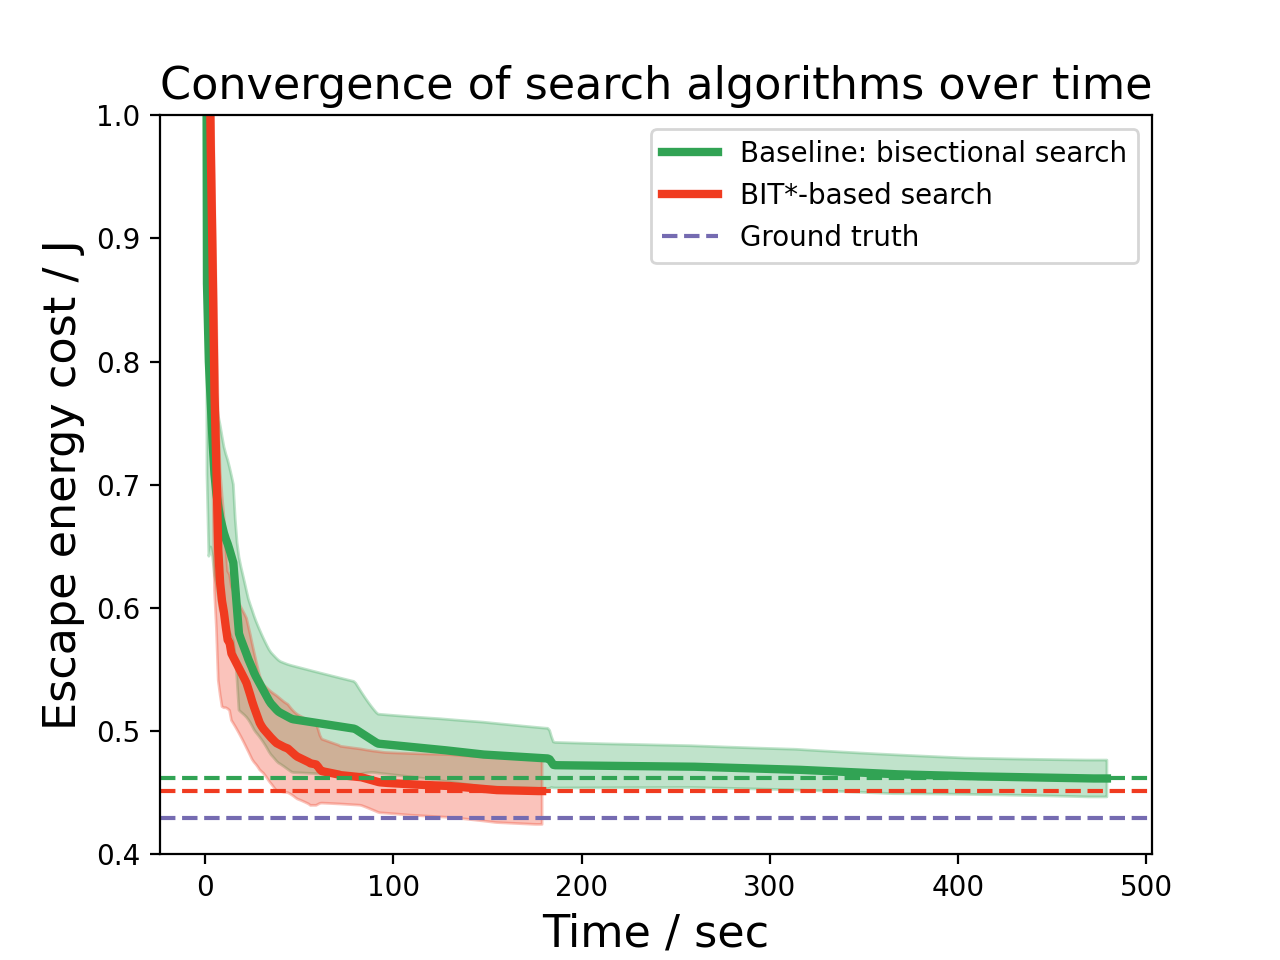
\includegraphics[width=0.7\linewidth]{figures/benchmark_convergence_keyframe18.png}}
	% \caption{Comparison of the BIT* and baseline for approximating escape energy for each frame of the ring-hook scenario (Figure \ref{fig1} top) shows near identical numerical values. 
		% The calculated escape energy (as approximated using the BIT*-based and incremental planner) for each frame $i$ (left) is nearly identical for both methods. Convergence of the algorithms over time (right) at frame 18 (corresponding to the vertical dashed line, and a ring configuration $\boldsymbol{\xi}_{18}$ corresponding to B in the top of Figure \ref{fig1}) indicates superior performance by BIT*.
		% Escape energy is estimated using 6 independent runs of a 3-min execution of the BIT*-based approach, and an 8-min incremental search as the baseline.
		% The horizontal dashed lines (red and green) indicate the terminal approximation value of escape energy by running BIT* and the baseline, respectively.
		% %\vspace{-8pt}
		% }
	% \label{fig2}
	% \vspace{-10pt}
	% \end{figure}

\subsection{Quantitative Analysis}
% \begin{enumerate}
	%     \item BIT*, incremental and binary search compared with reference in the ring-hook scenario.
	%     \item Runtime vs Accuracy (relative error of escape energy w.r.t ground truth) using BIT*
	%     \item Comparison of using various planners, RRT*, BIT*, ...
	%     \item Runtime analysis within a search (collision detection, etc.)
	%     \item Modeling precision (no. of DoF) vs precision in the band-hourglass example
	% \end{enumerate}
We empirically verify the accuracy and efficiency of our proposed approaches in Fig. \ref{} with the scenario of a rigid ring swinging on a hook (Fig. \ref{}).
BIT* appears to result in a very similar accuracy as compared to the iterative methods over dozens of frames, and they are all close to the reference escape energy, which indicates a high level of accuracy in a 6 DoF C-space.
We observe an improved convergence speed of BIT* over the other two within 10min runtime.
The convergence of the binary search depends heavily on where the true escape energy $\bar{u}$ lies within the interval of initial energy lower and upper bounds $[u_-^0,u_+^0]$.
$\bar{u}$ closer to $u_-^0$ clearly leads to faster convergence of the algorithm since the target is always within the search range in the first few iterations.
We also tested the accuracy in terms of state space dimensionality in a simple scenario of an elastic hair tie escaping from a human wrist (modeled by a conical frustum) as in Fig. \ref{}.
The hair tie is modeled by 3-9 control points, corresponding to 7-19 DoF in C-space.
The absolute error between escape energy and the reference increases in terms of higher dimensions and a quadratic energy function as in Eq. \ref{eq2}. 
\subsection{Qualitative Evaluation of Approximated Escape Energy}

\begin{enumerate}
	\item Scooping a fish with a shovel
	\item Hooking a frozen fish with a fishing hook
	\item Wearing a mask with two fingers
	\item Catching a starfish with a bowl
	\item Manipulating a rubic cube with two grippers
	\item Tying a bunch of radishes with a rubber band
	\item Grasping a chain of blood bags
	\item 2D snaplock
	\item Quick release snaplock for key chains
\end{enumerate}

The evaluation scenarios present examples of dynamic soft fixtures in the course of hooking an object, catching it with a bowl and a transition from soft fixture to caging for the starfish example. 
We simulate the objects' trajectories under gravity and potential energy using Pybullet (see the video and Fig.\ref{fig1}).
In Pybullet, the objects freely fall under gravity and are caught by fixed obstacles (bowl, hook, gripper) afterwards. The object configurations $\boldsymbol{\xi}_{i}$ ($i=0,1,...$) for each frame are recorded in this process and we analyze each such configuration in a quasi-static manner using our BIT*-based approach to approximate the required escape energy -- kinetic energy is ignored in the analysis, but present in the Pybullet simulation. We run 5 independent runs of a 2-min execution of the BIT*-based escape energy approximation for this purpose. 

In the ring-hook example (Figure \ref{fig1} top), a rigid ring with 1 N gravitational force falls (subfigure A) and is caught by the fixed fish hook (B).
We observe that its escape energy is initially zero as a sidewards translation and ring rotation around the center of mass provides an escape path that does not raise potential energy in the initial frames. After that, it enters a soft fixture (e.g. energy-bounded cage under gravity here) with estimated required escape energy reaching about 1 J as the hook's center of gravity falls deep below the tip of the hook. As the ring is suspended from the hook, it swings back and forth (C, D) due to kinetic energy present in the simulation - this results in an oscillation in our quasi-static escape energy analysis with a local minimum around C and local maximum around D as energy is stored in kinetic and potential energy during this swinging which is coming to rest over time resulting in a stabilizing non-zero escape energy.


In the previous example, we consider rigid objects such as the hook as a special case of articulated objects with zero elastic potential energy and  $l = 1, j = 0$. Next, we consider a simple articulated fish model approximation with $l = 12, j = 11$, see the bottom part of Fig.\ref{fig1}. As the fish falls (A) it initially can be pulled arbitrarily far away from its current configuration without raising potential energy, however, it then hits the rim of the bowl and pivots around the contact point (B). Around this time, the required escape energy starts to rise and the elastic potential energy is non-zero due to the deformation caused by the collision with the rim and the pull of gravity.
The fish slides down slowly (C, D) along the inner wall of the bowl, and its curvature and elastic potential energy are constrained by the curvature of the bowl.
We also observe that a configuration with maximum energy
%$ \boldsymbol{\xi}^{*}_{max} = 
%\sigma^{*}(\argmax_{\theta \in [0,1]} E(\sigma^{*}(\theta)))$
along an optimal escape path appears to lie in the vicinity of (1) the tip of the fish hook with the ring dangling from it, and (2) the rim of the bowl with the fish body slightly bent downward respectively.
%, to guarantee minimum energy and sliding through the obstacle borders when $z_{s}(\bxi_{init})$ is below the tip or the rim.

\subsection{Real Experiment}

\section{Conclusion}
In this paper, we provide a perspective on restraining deformable objects in the configuration space by extending the concept of energy-bounded caging to a high-dimensional space.
We have demonstrated escape energy approximation of soft fixtures with complex gravitational and elastic potential energy constraints can in principle be studied using the proposed sampling-based methods.
The work generalizes caging-based manipulation towards more practical ends.
The approach is, nevertheless, limited in a way that the probability of escape is not solely affected by escape energy, but also obstruction clearance such as narrow passages in the workspace.
Quasi-static planning along escape paths also ignores some complex dynamics and frictions in reality.
However, future work based on our work that considers gripper C-space planning in combination with the object escape planning is promising.
The dimensionality curse of the composite C-space can be tackled by learned latent space planning \cite{} or learned representation of deformable objects \cite{}.

% https://ieeexplore.ieee.org/stamp/stamp.jsp?arnumber=8653875 Robot Motion Planning in Learned Latent Spaces
% Modeling, learning, perception, and control methods for deformable object manipulation, H Yin, A Varava, D Kragic

% \section{Random Thoughts}
% Two catalogs: direct manipulation by robot grippers and tool-in-hand manipulation. We wanted to stress the importance of the latter since dexterous tools provide the possibility of more complicated manipulation that a bare human hand cannot achieve.
% An interesting observation is that in some manipulation cases, it is the tool that is caged or fixtured instead of objects that are desirably manipulated (2D snap lock and coriander example). 

% with string-like properties or isotropic deformable objects.  
% such as masks, isotropic deformable objects like meat, and other related experiments in real-world scenarios.
% Our future directions include building a large-scale dataset of caging for deep learning using the offline sampling-based approach we propose. 
% We also plan to explore caging planning of particle-based deformable objects in the latent space.


\balance
\begin{thebibliography}{00}
	\bibitem{b18} A. Bicchi and V. Kumar, "Robotic grasping and contact: a review," IEEE International Conference on Robotics and Automation. 2000, pp. 348-353 vol.1.
	\bibitem{b19} J. C. Trinkle, J. M. Abel, and R. P. Paul, "An Investigation of Frictionless Enveloping Grasping in the Plane," in IEEE International Journal of Robotics Research, vol. 7, no. 3, pp. 33-51, Jun. 1988.
	\bibitem{b20} V. D. Nguyen, "Constructing Force-Closure Grasps," in IEEE International Journal of Robotics Research, vol. 7, no. 3, pp. 3-16, Jun. 1988.
	\bibitem{b1} W. Kuperberg, "Problems on polytopes and convex sets," in Proceedings of DIMACS: Workshop on Polytopes, 1990, pp. 584-589.
	\bibitem{b2} E. Rimon and A. Blake, "Caging 2D bodies by 1-parameter two-fingered gripping systems," Proceedings of IEEE International Conference on Robotics and Automation, 1996, pp. 1458-1464 vol.2.
	\bibitem{b3} E. Rimon and A. Blake, "Caging planar bodies by one-parameter two-fingered gripping systems," International Journal of Robotics Research, vol. 18, pp. 299-318, 1999.
	\bibitem{b4} T. F. Allen, J. W. Burdick and E. Rimon, "Two-Finger Caging of Polygonal Objects Using Contact Space Search," in IEEE Transactions on Robotics, vol. 31, no. 5, pp. 1164-1179, Oct. 2015.
	\bibitem{b5} T. F. Allen, E. Rimon and J. W. Burdick, "Two-finger caging of 3D polyhedra using contact space search," 2014 IEEE International Conference on Robotics and Automation (ICRA), 2014, pp. 2005-2012.
	\bibitem{b7} A. Rodriguez, M. T. Mason, and S. Ferry, "From caging to grasping," The Int. Journal of Robotics Research, vol. 31, no. 7, pp. 886-900, Jul. 2012.
	\bibitem{b9} F. T. Pokorny, J. A. Stork and D. Kragic, "Grasping objects with holes: A topological approach," 2013 IEEE International Conference on Robotics and Automation, 2013, pp. 1100-1107.
	\bibitem{b8} A. Varava, D. Kragic and F. T. Pokorny, "Caging Grasps of Rigid and Partially Deformable 3-D Objects With Double Fork and Neck Features," in IEEE Transactions on Robotics, vol. 32, no. 6, pp. 1479-1497, Dec. 2016.
	\bibitem{b12} J. Mahler, F. T. Pokorny, Z. McCarthy, A. F. van der Stappen and K. Goldberg, "Energy-Bounded Caging: Formal Definition and 2-D Energy Lower Bound Algorithm Based on Weighted Alpha Shapes," in IEEE Robotics and Automation Letters, vol. 1, no. 1, pp. 508-515, Jan. 2016.
	\bibitem{b13} J. Mahler, F. T. Pokorny, S. Niyaz and K. Goldberg, "Synthesis of Energy-Bounded Planar Caging Grasps Using Persistent Homology," in IEEE Transactions on Automation Science and Engineering, vol. 15, no. 3, pp. 908-918, July 2018.
	\bibitem{x1} A. Varava, J. F. Carvalho, D. Kragic, F. T.  Pokorny, "Free space of rigid objects: Caging, path non-existence, and narrow passage detection", The international journal of robotics research 40.10-11 (2021): 1049-1067.
	\bibitem{b22} H. D. Young and R. A. Freedman, "University Physics with Modern Physics," 13th ed., Pearson Education, Inc., 2012.
	\bibitem{b15} S. LaValle and J. Kuffner Jr., "Randomized kinodynamic planning," in Proceedings 1999 IEEE International Conference on Robotics and Automation, 1999, pp. 473-479.
	\bibitem{b11} A. Varava, M. C. Welle, J. Mahler, K. Goldberg, D. Kragic and F. T. Pokomy, "Partial Caging: A Clearance-Based Definition and Deep Learning," 2019 IEEE/RSJ International Conference on Intelligent Robots and Systems, 2019, pp. 1533-1540.
	\bibitem{b14} J. D. Gammell, S. S. Srinivasa and T. D. Barfoot, "Batch Informed Trees (BIT*): Sampling-based optimal planning via the heuristically guided search of implicit random geometric graphs," 2015 IEEE International Conference on Robotics and Automation, 2015, pp. 3067-3074.
	\bibitem{b16} J. D. Gammell, T. D. Barfoot, and S. S. Srinivasa, "Batch Informed Trees (BIT*): Informed asymptotically optimal anytime search," The International Journal of Robotics Research, vol. 39, no. 5, pp. 543-567, Apr. 2020.
	\bibitem{b17} D. Devaurs, T. Siméon and J. Cortés, "Optimal Path Planning in Complex Cost Spaces With Sampling-Based Algorithms", in IEEE Transactions on Automation Science and Engineering, vol. 13, no. 2, pp. 415-424, April 2016.
	\bibitem{R1} M. Bourgeois, O. Grenier, and S. Bélanger, "The Robotiq 3-Finger Gripper: A Versatile End-Effector for Industrial Robots," in IEEE Robotics Automation Magazine, vol. 23, no. 4, pp. 71-82, Dec. 2016.
	\bibitem{o1} M. Otte, R. Alterovitz, D. Ferguson, L. E. Kavraki, and J. T. Betts, “Open Motion Planning Library: A planning and control toolbox for motion planning,” in Proceedings of the IEEE International Conference on Robotics and Automation (ICRA), pp. 5422–5429, May 2013.
	\bibitem{o2} E. Coumans and Y. Bai, "PyBullet, a Python module for physics simulation for games, robotics and machine learning," [Online]. Available: http://pybullet.org, 2016-2021.
	
	% \bibitem{b21} N. C. Dafle et al., "Extrinsic dexterity: In-hand manipulation with external forces," 2014 IEEE International Conference on Robotics and Automation, 2014, pp. 1578-1585.
	% \bibitem{b6} S. Makita, W. W. Wan, "A survey of robotic caging and its applications," Advanced Robotics, 31(19-20), pp. 1071-1085, 2017.
	\bibitem{b10} T. Makapunyo, T. Phoka, P. Pipattanasomporn, N. Niparnan, and A. Sudsang, “Measurement framework of partial cage quality,” in ROBIO, 2012
	
	
	
	
\end{thebibliography}
\vspace{12pt}
\color{red}

% \begin{figure*}[htbp]
	% \centerline{\includegraphics[width=0.8\textwidth]{figures/ICRAfigure_hook2.png}}
	% \caption{
		% Plotted are the total potential energy (in green), and the minimum of the escape energy costs (in red) of the per-frame quasi-static caging analysis of the scenarios by running 5-time 2-min BIT*-based motion planning for each datapoint.
		% % Each iteration is repeated 5 times independently.
		% % the green curves denote the total potential energy of the caged objects, the red curves the minimum of escape energy costs over $6$ runs, with
		% The plus/minus one standard deviation of the escape energy costs extends from its mean (not plotted since we care about the minimum only, which is closest to and upper-bounds the optimal escape energy costs $u^* = V(\sigma^*) $) in red shadings. 
		% }
	% \label{fig}
	% \end{figure*}

% \begin{figure*}[htbp]
	% \centerline{\includegraphics[width=0.8\textwidth]{figures/ICRAfigure_fish.png}}
	% \caption{
		% The scenario of fish falling into a bowl.
		% Additional curves of the gravitational and the elastic potential energy (in purple and blue, respectively) are included.
		% }
	% \label{fig}
	% \end{figure*}

\end{document}
